\documentclass[10pt,a4paper]{article}

\usepackage{fontspec}
\usepackage{csquotes}
\usepackage[ngerman]{babel}
\usepackage[colorinlistoftodos]{todonotes}
\usepackage[backend=biber,style=numeric]{biblatex}
\usepackage{graphicx}
\usepackage{float}
\usepackage{wrapfig}
\usepackage{amsmath}
\usepackage{commath}
\usepackage{gensymb}
\usepackage{listings,xcolor,gnuplottex}

% Space savings:
\usepackage[top=2.5cm, left=2.5cm, right=2.5cm, bottom=2cm]{geometry}
\setlength\parindent{0pt}
%\usepackage[subtle]{savetrees}

% Mathematica listening
\lstset{language=Mathematica} % mathmatica snippets
\lstset{basicstyle={\sffamily\footnotesize},
  numbers=left,
  numberstyle=\tiny\color{gray},
  numbersep=5pt,
  breaklines=true,
  captionpos={t},
  frame={lines},
  rulecolor=\color{black},
  framerule=0.5pt,
  columns=flexible,
  tabsize=2
}

\addbibresource{bib.bib}

\title{Akustische Richtungsbestimmung}
\author{Robin Heinemann\\ Jaro Habiger}
\date{\today}

\begin{document}
  \maketitle
  \begin{abstract}\todo{write me!!}
  \end{abstract}
  \thispagestyle{empty}
  
  \newpage
  \tableofcontents
  \thispagestyle{empty}
  
  \newpage
  \setcounter{page}{1}
  %begin the content

  \begingroup
    \let\clearpage\relax
    \section{Problematik}\todo{wir wollen offenes Verfahren -> es könne Amplituden,... eingebaut werden}
\todo{Durchlesen + überprüfen}
Der Mensch hat die Fähigkeit, direktional zu hören, also die Richtung zu bestimmen aus der ein Geräusch kommt. Dies bringt ihm enorme Vorteile bei der Erkennung von gesprochener Sprache und bei anderen akustischen Aufgaben. Diese Fähigkeit auf eine technische Apparatur zu übertragen und die Vorteile des räumlichen Hörens auch für diese nutzbar zu machen, hätte viele Anwendungsgebiete, die unser alltägliches Leben erleichtern könnten.\\
Ein gutes Beispiel für eine Solche Anwendung wäre ein Rettungsroboter, der Hilfesuchende Menschen anhand von Hilferufen lokalisiert. Auch könnte man verschiedene Hilfsmittel für den Menschen Konstruieren, die ein solches technisches Verfahren verwenden. Ein Beispiel hierfür wäre ein Helm, den sich Feuerwehrleute aufsetzen können um in verrauchten Umgebungen Geräuschen wie schreienden Babys zu folgen.\\
Jedoch sind auch Anwendungen aus komplett anderen Anwendungsbereichen denkbar: So wäre es möglich eine Anwendung zu entwickeln, die die Richtungsinformationen verwendet, um Audiosignale zu filtern. Hiervon würde zum Beispiel die Spracherkennung profitieren, da sie sehr störungsfreie Audiosignale benötigt und immer nur ein Sprecher von Interesse ist\cite{Spracherkennung}. Auch andere Anwendungen, die störungsfreie Audiosignale b benötigen, könnten die Vorteile der Richtungserkennung nutzen. 

    \section{Bestehende Lösungen} \todo{Die anderen mehr Bashen!}
  Es gibt einige bestehende Ansätze, die die verschiedenen Aspekte des direktionalen Hörens auf eine technische Apparatur übertragen. Diesen begegnen wir in unserem alltäglichen Leben relativ häufig. Die einfachste Form eines solchen Verfahrens ist das Richtmikrofon. Dieses führt allerdings keine aktive Ortung durch, sondern kann lediglich in eine bestimmte Richtung besonders gut Schall aufnehmen. Um diese Fähigkeit für eine Richtungsbestimmung zu nutzen, müsste man also das Richtmikrofon drehen, oder es auf eine andere Weise aktiv nach der Schallquelle ausrichten. Ein weiterer Ansatz, dem wir in unserem alltäglichen Leben noch sehr viel häufiger begegnen, steckt in fast allen Mobiltelefonen. Diese filtern beim Telefonieren verschiedene Umgebungsgeräusche aus dem Mikrofonsignal, um die Sprachqualität zu verbessern. Die hierzu verwendeten Verfahren sind allerdings meist eher einfach gehalten und erlauben keine wirkliche Bestimmung der Herkunftsrichtung eines Geräusches. Man kann sich dieses Verfahren sehr gut als ein Richtmikrofon vorstellen, das einen gewissen Bereich hat, in dem es sehr empfindlich ist, wohingegen es in anderen Bereichen sehr unempfindlich ist. Bei dieser Technik passiert ein Teil der Geräuschunterdrückung in der Signalverarbeitung, also nach der eigentlichen Schallwandlung durch das Mikrofon. Hierdurch unterscheidet sich dieser Ansatz deutlich von dem des Richtmikrofones. Allerdings können auch mithilfe dieser Störgeräuschunterdrückung noch keine Positionen ermittelt werden. Auch moderne Hörgeräte verwenden ein ähnliches Verfahren, welches allerdings auch bei einer weiteren Distanz zwischen Mikrofon und Schallquelle funktioniert, und der gesuchten Lösung somit näher kommt. Sowohl die Geräuschunterdrückung in Handys, als auch die Filtertechniken in Hörgeräten verwenden meist zwei oder drei Mikrophone.
  \begin{figure}
    \centering
    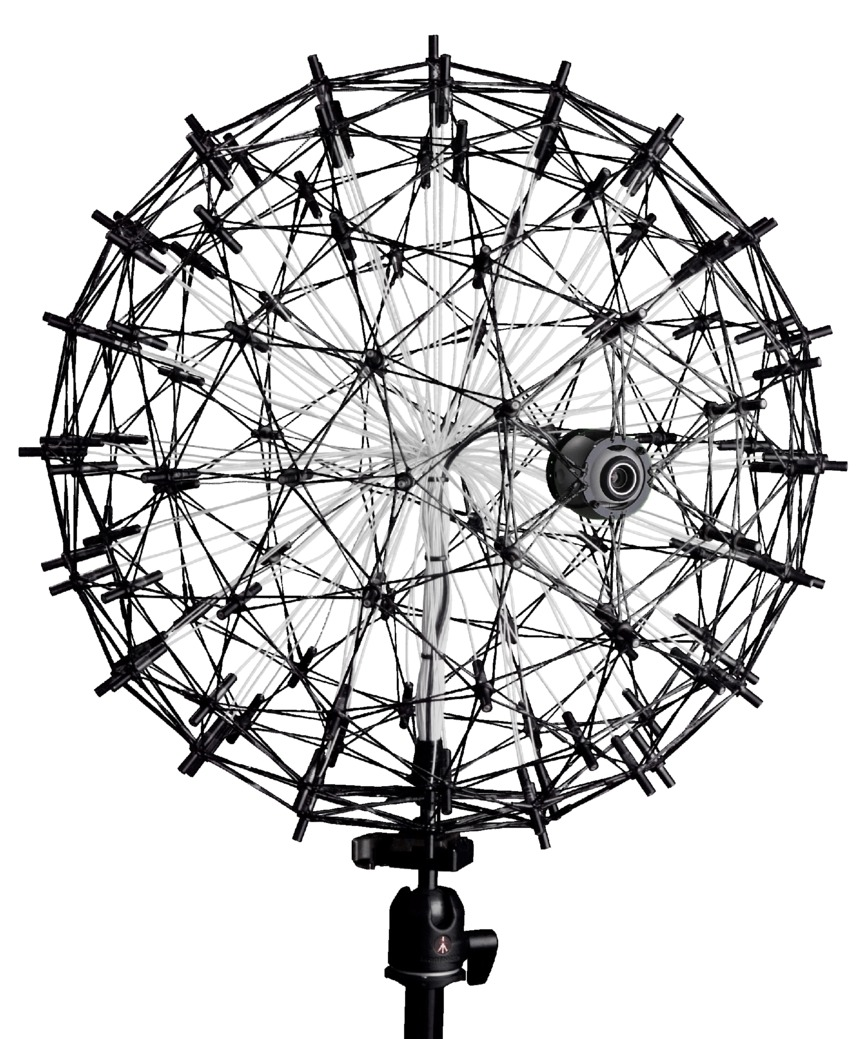
\includegraphics[width=0.35\linewidth]{img/akusticCamera}
    \caption{Ein Beispiel für eine akustische Kamera \cite{camera}}
    \label{fig:camera}
  \end{figure}
  Eine andere existierende Lösung ist die akustische Kamera (siehe Abb. \ref{fig:camera}). Sie wird dazu verwendet, lärm-emittierende Positionen an Produkten zu finden, um diese optimieren zu können \cite{camera}. Die akustische Kamera verwendet allerdings bedeutend mehr Mikrofone als die anderen Verfahren. Einige Modelle verwenden mehr als 350 Mikrofone \cite{nmics}.\todo{warum ist akust. Kamera nicht die Lösung: Ist auf best. Produkte gemünzt} Da uns alle vorhandenen Lösungen nicht zufrieden gestellt haben, wollten wir ein eigenes Verfahren für die akustischen Richtungsbestimmung entwickeln, das schon mit einer geringen Anzahl von Mikrofonen eine komplette Richtungsbestimmung ermöglicht und leicht erweiterbar auf weitere Auswertungsschritte ist.

    \section{Konzept}
Bei der Entwicklung unseres neuen Verfahrens zur Richtungsbestimmung haben wir uns stark am menschlichen Gehör und seiner Fähigkeit des Richtungshörens orientiert. Da beim menschlichen Gehör verschiedene Verarbeitungssstufen durchlaufen werden, ist auch unsere Software modular aufgebaut (siehe Tabelle \ref{analog}). Nachfolgend werden die einzelnen Module in der Reihenfolge, in der das Signal sie durchläuft, beschrieben.
Um unser Konzept umzusetzen und zu evaluieren, haben wir uns entschlossen, einerseits eine Computersimulation zu schreiben und andererseits mithilfe einer realen Messapparatur zu überprüfen, ob unser Verfahren auch in der Echtwelt verwendbar ist. Der reale Aufbau soll zuerst in einer Schallkammer, also einem Raum mit wenigen akustischen Störquellen von außen und mit wenigen akustischen Reflexionen an den Wänden, und erst danach unter Einfluss von Störungen getestet werden. Dieses Vorgehen hat den Vorteil, dass man zuerst die Theorie entwickeln kann, und danach die Theorie und ihre Implementation in den verschiedenen Schritten zum Endprodukt immer weiter an Realwelteffekte, wie zum Beispiel Rauschen, anpassen kann. Auch hierbei hilft der modulare Aufbau, da so möglichst viele Programmteile sowohl in der Simulation, als auch in realen Aufbauten verwendet werden können.
Unser Konzept sieht vier Module vor, welche über TCP/IP und Websockets verbunden sind. Dies sind Standards, mit denen über ein Computernetzwerk Daten ausgetauscht werden können \cite{tcp} \cite{websockets}. Diese beiden Protokolle sind sehr zuverlässig und lange erprobt. Außerdem garantieren sie, dass alle Daten in der Reihenfolge, in der sie losgeschickt werden, ankommen. Die Verwendung von Netzwerkprotokollen hat den Vorteil, dass die Module nicht unbedingt auf demselben Computer ausgeführt werden müssen und so der Rechenaufwand bei Bedarf auf mehrere Computer verteilt werden kann.
\begin{table}[h]
	\centering
	\begin{tabular}{ll}
		Mensch            & Unser Verfahren                                   \\ \hline
		Ohren             & Mikrofonarray                              \\
		Haarzellen im Ohr & Fourier Transformation                     \\
		Richtungsbestimmung im Gehirn            & Computeralgorithmus zur Richtungsbestimmung                       \\
		Selektives Hören  & Weiterverarbeitung durch Programme Dritter
	\end{tabular}
	\caption{Die Analogie zwischen dem menschlichen Gehör und unserem Verfahren}
	\label{analog}
\end{table}

\subsection{Modul 1: Eingabe/Aufnahme}
Das erste Modul in dieser Kette stellt die Rohdaten für die weitere Verarbeitung bereit. Diese  können entweder von einer Gruppe real existierender Mikrofone stammen oder, im Falle der Simulation, die Signale einer Gruppe simulierter Mikrofone, die simulierte Schallquellen aufnehmen, sein. Dieses Modul entspricht dem menschlichen Ohr und seiner Aufgabe, den Schall aufzunehmen. 

\subsection{Modul 2: Signal nach Frequenzen aufteilen}
Im zweiten Modul der Kette wird das Signal, welches aus dem ersten Modul stammt, in die einzelnen im Signal enthaltenen Wellen aufgeteilt, also von einer zeitaufgelösten Form in ein frequenzaufgelöstes Signal umgewandelt. Nach diesem Schritt liegt also für jede Frequenz eine Amplitude und eine Phase vor. Dieser Schritt wird im menschlichen Ohr durch eine mechanische Konstruktion, die verschiedene Haarzellen für verschiedene Frequenzen anregt, vorgenommen. Unser technisches Verfahren verwendet hierzu die Fouriertransformation. Diese Transformation hat den Vorteil, dass jede Frequenz mit ihrer zugehörigen Amplitude und Phase einzeln analysiert werden kann.
In diesem Modul werden außerdem Frequenzen, welche nicht oder nur sehr leise in dem Eingangssignal vorkommen, herausgefiltert, um das Rauschen und den benötigten Rechenaufwand in den nächsten Modulen zu verringern.

\subsection{Modul 3: Richtungsbestimmung}
Das nächste Modul empfängt die Daten des vorherigen Moduls und errechnet zunächst für jede Frequenz aus den transformierten Daten den Gangunterschied zwischen den Signalen der Mikrofone. Aus diesen werden dann die möglichen Ursprungsrichtungen der einzelnen Sinusschwingung ermittelt. Da dieser Vorgang für jede Frequenz einzeln vorgenommen wird, können auch mehrere Schallquellen mit unterschiedlichen Frequenzen gleichzeitig untersucht werden. Im menschlichen Gehör wird diese Richtungsbestimmung im Gehirn vorgenommen.

\subsection{Modul 4: Ausgabe}
Das letzte Modul in der Signalkette ist die Ausgabe. Sie bekommt die fertig gruppierten Messergebnisse über eine Netzwerk-Verbindung und bereitet sie für den Nutzer auf. Dieses Modul kann auf die jeweilige Anwendung angepasst werden und es können mehrere Output-Module mit dem gleichen Richtungsmodul verbunden werden. Hier kann dann die Endanwendung, die das Richtungshören verwenden möchte, \textit{angeschlossen} werden.\\
Der Mensch kann sich zum Beispiel mithilfe der bestimmten Richtungen auf einzelne Schallquellen konzentrieren und andere Geräusche ausblenden.
    \section{Umsetzung der einzelnen Module}
Der Kern unserer Idee ist die Richtungsbestimmung, die aus den Phasendifferenzen der verschiedenen Wellen bei verschiedenen Mikrofonen eine Richtung berechnet. Um diese Komponente überprüfen und das Verfahren anwenden zu können, haben wir die verschiedenen Module implementiert (Siehe Abbildung \ref{fig:flowchart}). Hierbei haben wir diese wie vorgesehen so universell umgesetzt, dass wir das Richtungsbestimmungsmodul sowohl mithilfe einer Simulation als auch mithilfe eines praktischen Aufbaus evaluieren können. Das nachfolgende Kapitel beschreibt eben diese Umsetzung in der Reihenfolge, mit der das Signal verarbeitet wird; von der Aufnahme der Schallquellen bis zur Ausgabe der Positionsdaten.
\begin{figure}[H]
	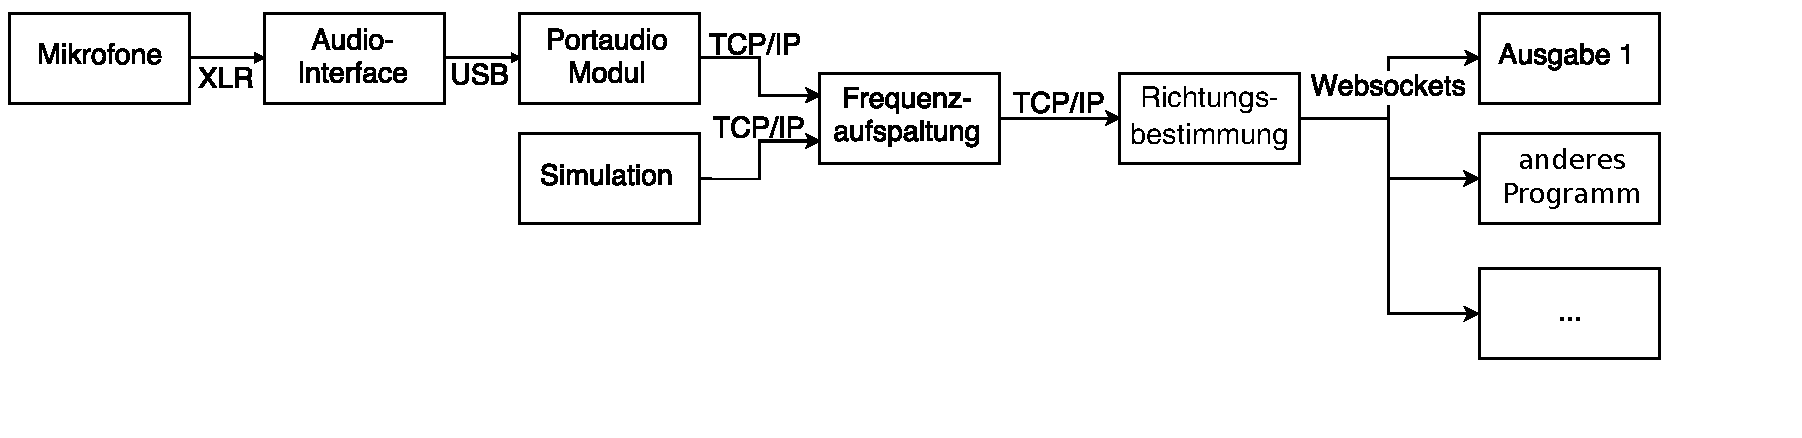
\includegraphics[width=\linewidth]{img/flowchart}
	\caption{Der modulare Aufbau unseres Konzeptes}
	\label{fig:flowchart}
\end{figure}

\subsection{Audiosimulation (Modul 1)}
Um die Richtungsbestimmung unabhängig von Störfaktoren wie dem Rauschen und der Reflexion des Schalls an Wänden oder anderen Gegenständen zu überprüfen, haben wir zunächst eine Simulation entwickelt. Außerdem lässt sich mit dieser gezielt der Einfluss verschiedener Störfaktoren untersuchen. Die Simulation kann beliebig viele Mikrofone an beliebigen Positionen simulieren. Leider konnten wir keine bestehenden Lösungen für die Simulation von dreidimensionalem Ton, wie \textit{OpenAL} \cite{OpenAL}, welches eine Programmbibliothek für die Simulation von Schall ist, verwenden, da bei diesen die Anzahl der Mikrofone limitiert ist und die Phase des Audiosignals in der Simulation vernachlässigt wird. Da die Funktion unserer Richtungsbestimmung unabhängig von den Amplituden der Schallquellen bei den einzelnen Mikrofonen ist, haben wir unsere Simulation rein auf die Phase und die Laufzeit beschränkt. Um eine interaktive Benutzung und eine leichte Überprüfung der Richtungsbestimmung zu gewährleisten, besitzt die Simulation eine graphische Benutzeroberfläche, mit der man interaktiv Schallquellen hinzufügen und entfernen kann. Außerdem kann die Simulation auch die bestimmten Richtungen darstellen und ermöglicht damit einen einfachen Vergleich der bestimmten und tatsächlichen Richtungen. Das Simulationsmodul wurde in der Programmiersprache \textit{C++} implementiert, da diese eine gute \textit{OpenGL} Integration bietet.

\begin{figure}[H]
	\centering
  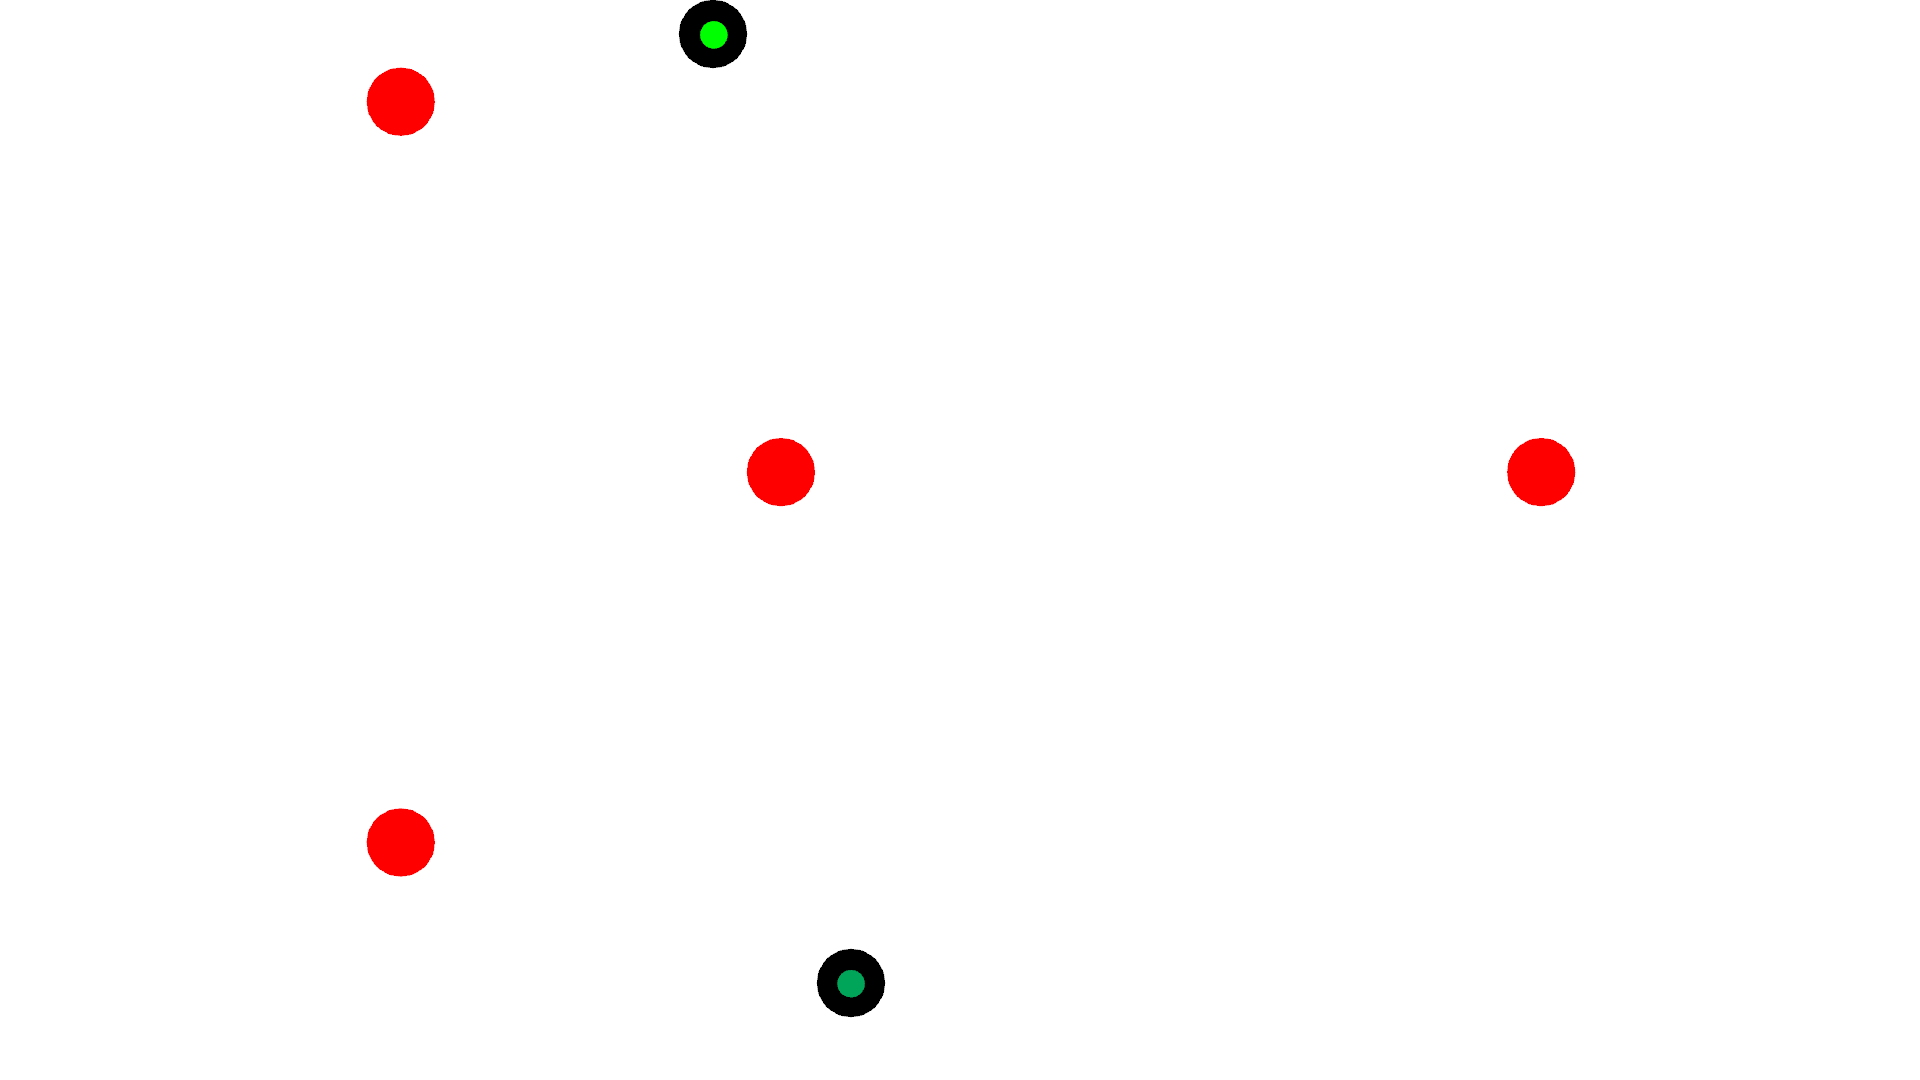
\includegraphics[width=(0.7\linewidth)]{img/bildsimulation}
  \caption{Screenshot der Simulation, die roten Punkte stellen die Mikrofone dar, die schwarzen die Schallquellen und die grünen die georteten Positionen}
\end{figure}

\subsection{Hardware (Modul 1)}
\begin{wrapfigure}{R}{0.4\textwidth}
	\centering
	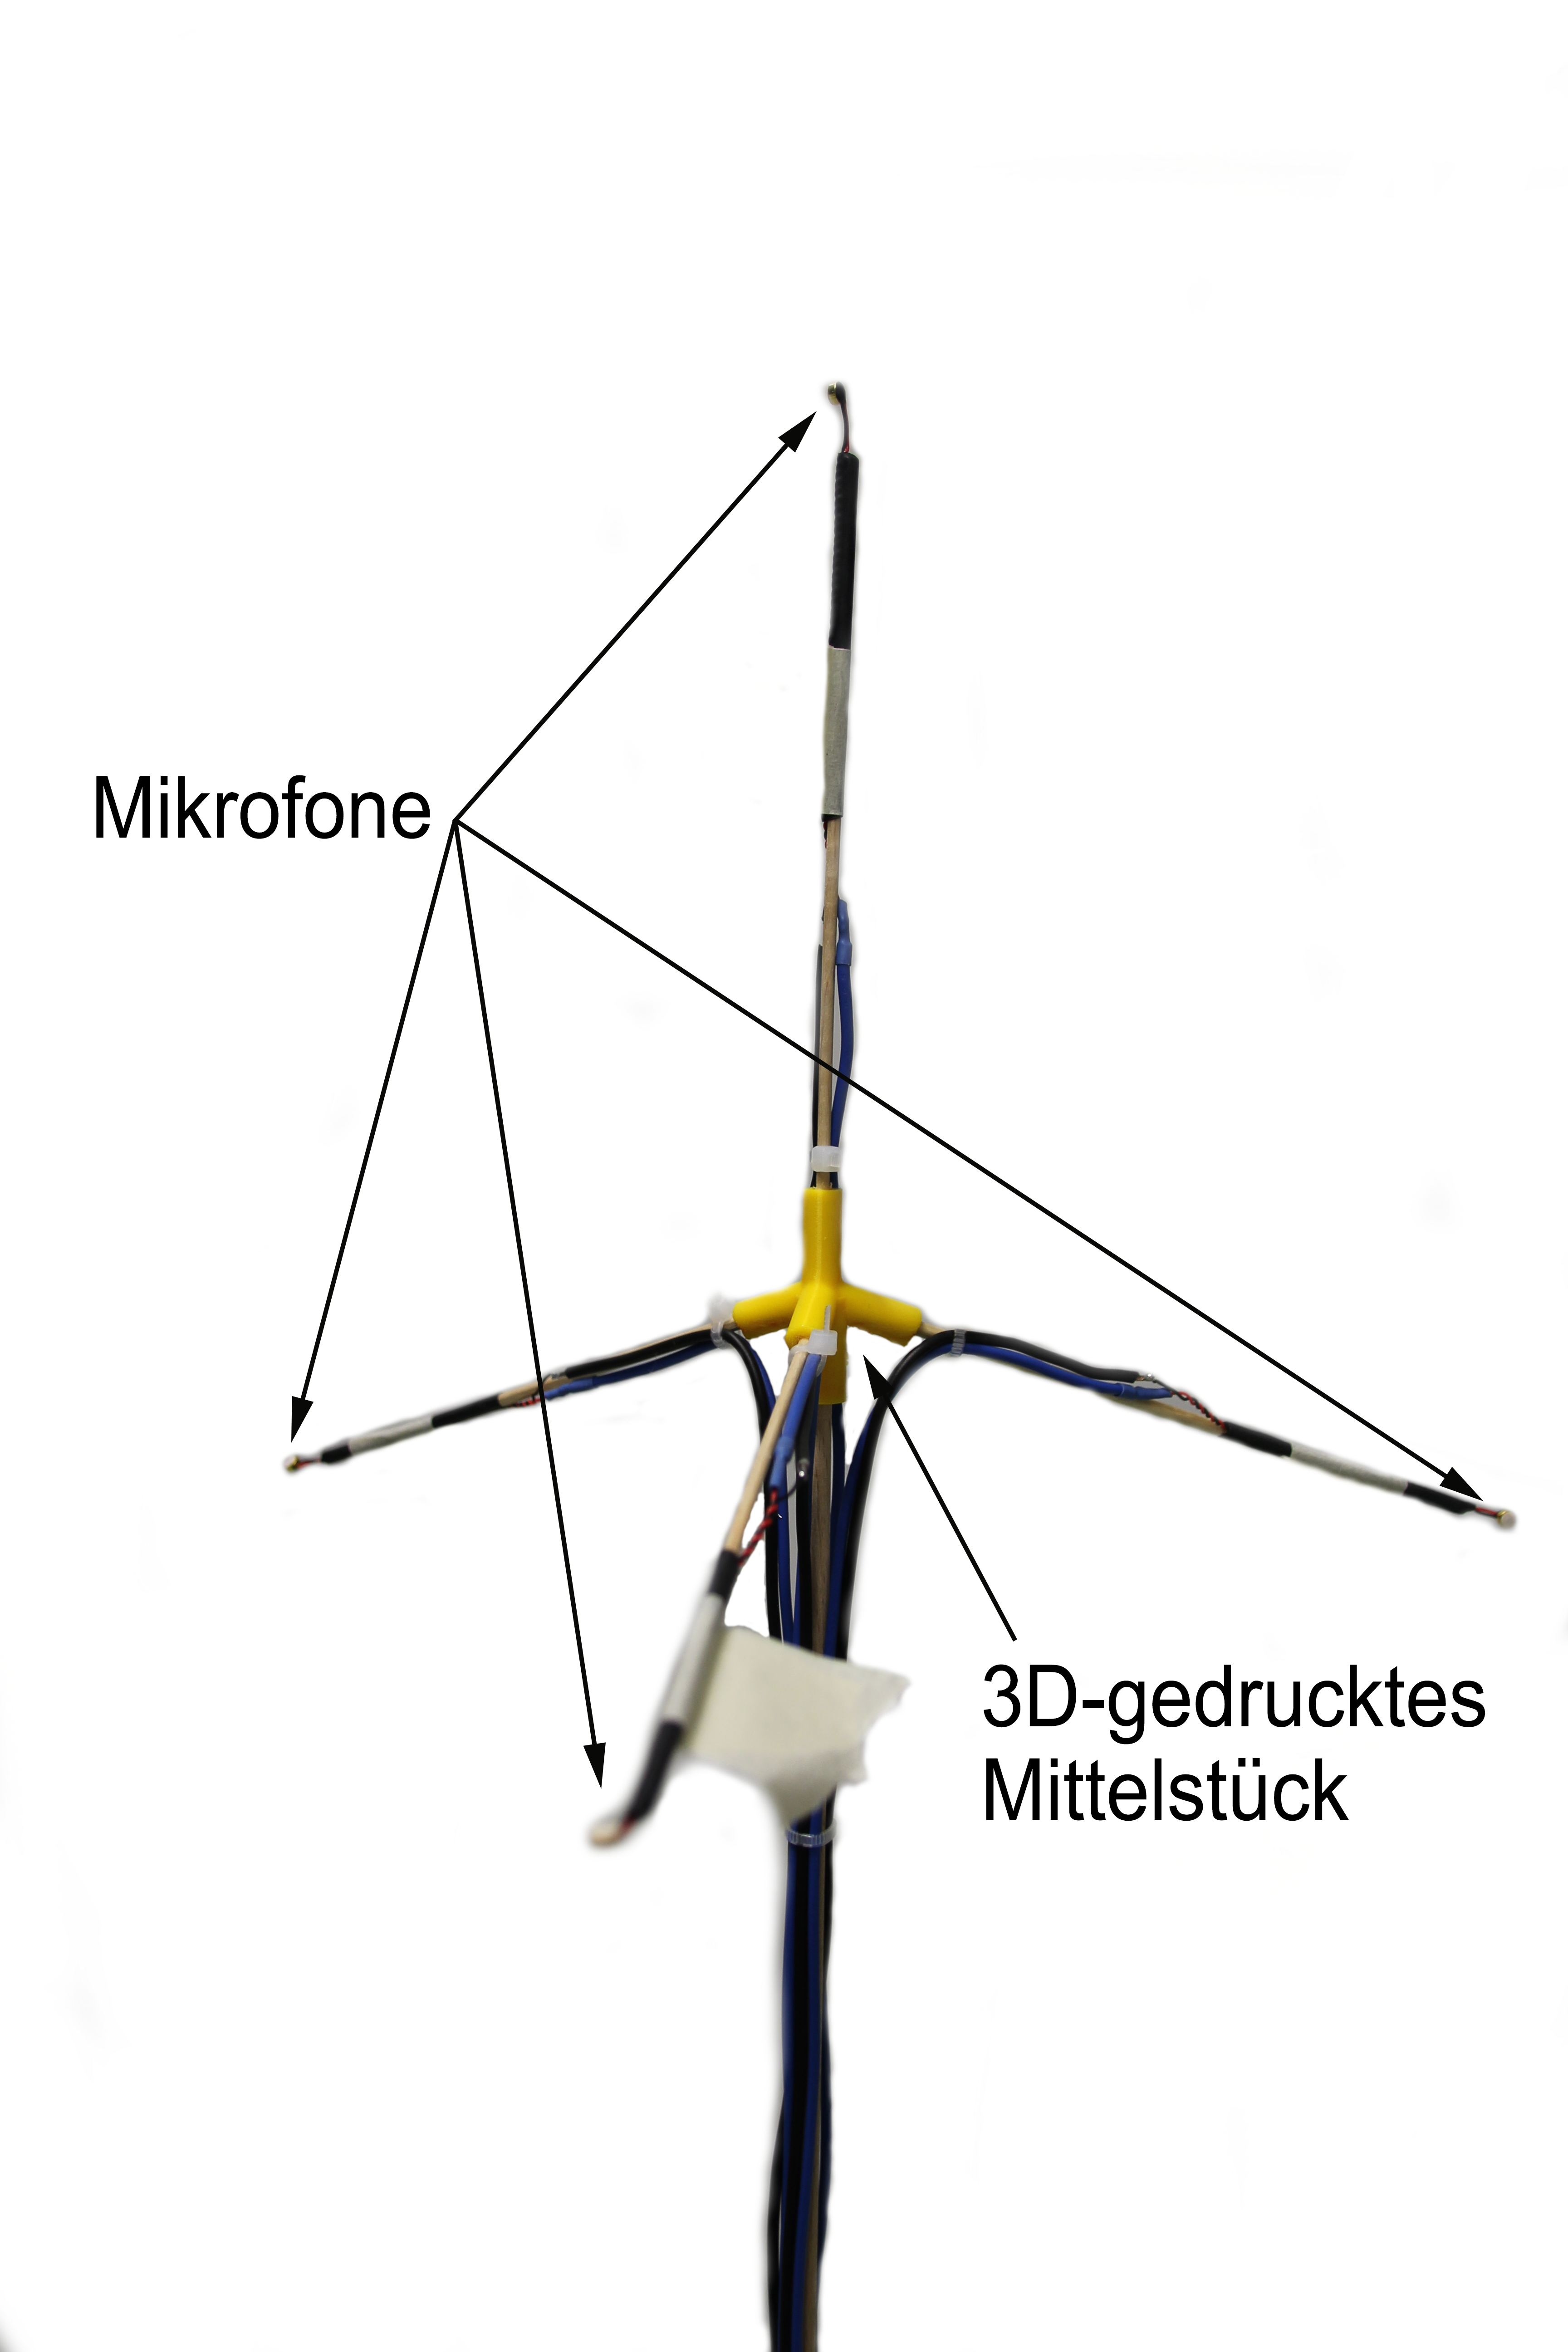
\includegraphics[width=\linewidth]{img/tet}
	\caption{Aufbau unserer Messapparatur}
\end{wrapfigure}
Um das durch die Simulation evaluierbare Verfahren praktisch zu testen und zu nutzen, muss nur die Quelle der Daten, also das erste Modul, ausgetauscht werden. Die Aufgabe des ersten Moduls ist es nun nicht mehr, virtuelle Mikrofone, welche die Aufnahme von virtuellen Schallquellen simulieren zu produzieren, sondern die Signale echter Mikrofone, welche echte Schallquellen aufnehmen, einzulesen. Um die Signale der Mikrofone mit einem Computer zu verarbeiten müssen sie digitalisiert werden. Zusätzlich benötigt man eine alternative Implementation der des ersten Moduls, die die Daten von der Hardware annimmt und an das zweite Modul weiterleitet. Hierbei kommen wieder die Vorteile unserer modularen Vorgehensweise zum tragen, da nur das erste Modul ersetzt werden muss und die gesamte restliche Software beibehalten werden kann. Dies sorgt auch dafür, dass die Simulation und die Realwelttests immer die gleichen Auswertungsalgorithmen verwenden und so sehr gut vergleichbar sind.
\subsubsection{Mikrofone}
Die erste Komponente, die es bei einem realen Aufbau der Messapparatur eine wichtige Rolle spielt, ist die der Schallwandlung. Dies wird durch Mikrofone realisiert, an die es einige Anforderungen gibt. Die wichtigste Anforderung ist, dass sie eine möglichst gleichmäßige Richtcharakteristik haben.
Eine weitere Anforderung ist, dass sie möglichst klein sind, da der Abstand zwischen ihnen nicht zu groß sein darf, um die obere Grenzfrequenz möglichst hoch zu setzen, da der Abstand der Mikrofone nicht größer als die Wellenlänge der zu lokalisierenden Frequenz sein darf. Des weiteren sollte das Signal-Rausch-Verhältnis möglichst groß sein, da Rauschen die Messungen unpräziser macht \cite{Rausch}.
Wir haben uns dafür entschieden, Elektretmikrofonkapseln zu verwenden, da diese üblich sind, keine aufwendige Elektronik zur Ansteuerung benötigen und die oben aufgeführten Anforderungen relativ gut erfüllen \cite{elektret}.
Die meisten für uns relevanten Parameter der Mikrofone konnten wir aus den Datenblättern entnehmen. Eine Ausnahme hiervon ist die Richtcharakteristik, welche jedoch für uns sehr wichtig ist, da sie die Messqualität sehr stark beeinflusst. Diese sollte möglichst gleichmäßig sein, da nur so aus allen Richtungen Daten von gleicher Qualität aufgenommen werden können. Wenn zum Beispiel alle Mikrofone eine Nierencharakteristik aufweisen und sie in einem gleichseitigen Dreieck angeordnet sind, liefert mindestens ein Mikrofon ein deutlich schwächeres Signal als die anderen, was dazu führt, das die Phasenlage der einzelnen Wellen ungenauer bestimmt werden und mit ihnen auch die Lokalisation ungenauer wird.
Um unter diesem Aspekt geeignete Mikrofone zu finden, haben wir die Richtcharakteristiken verschiedener Mikrofone mittels einer selbst entwickelten Messapparatur und einer selbst entwickelten Messsoftware vermessen. Die hierfür entwickelte Messapparatur sendet mittels eines Lautsprechers eine Sinus-Schwingung aus und misst, wie stark diese vom Mikrofon aufgenommen wurde. Danach dreht sie das Mikrofon um einen festgelegten Winkel weiter und fertigt erneut eine Messung an. Dieser Vorgang wird solange wiederholt, bis das Mikrofon einmal um 360$^{\circ}$ gedreht wurde.
\begin{figure}[H]
  \centering
  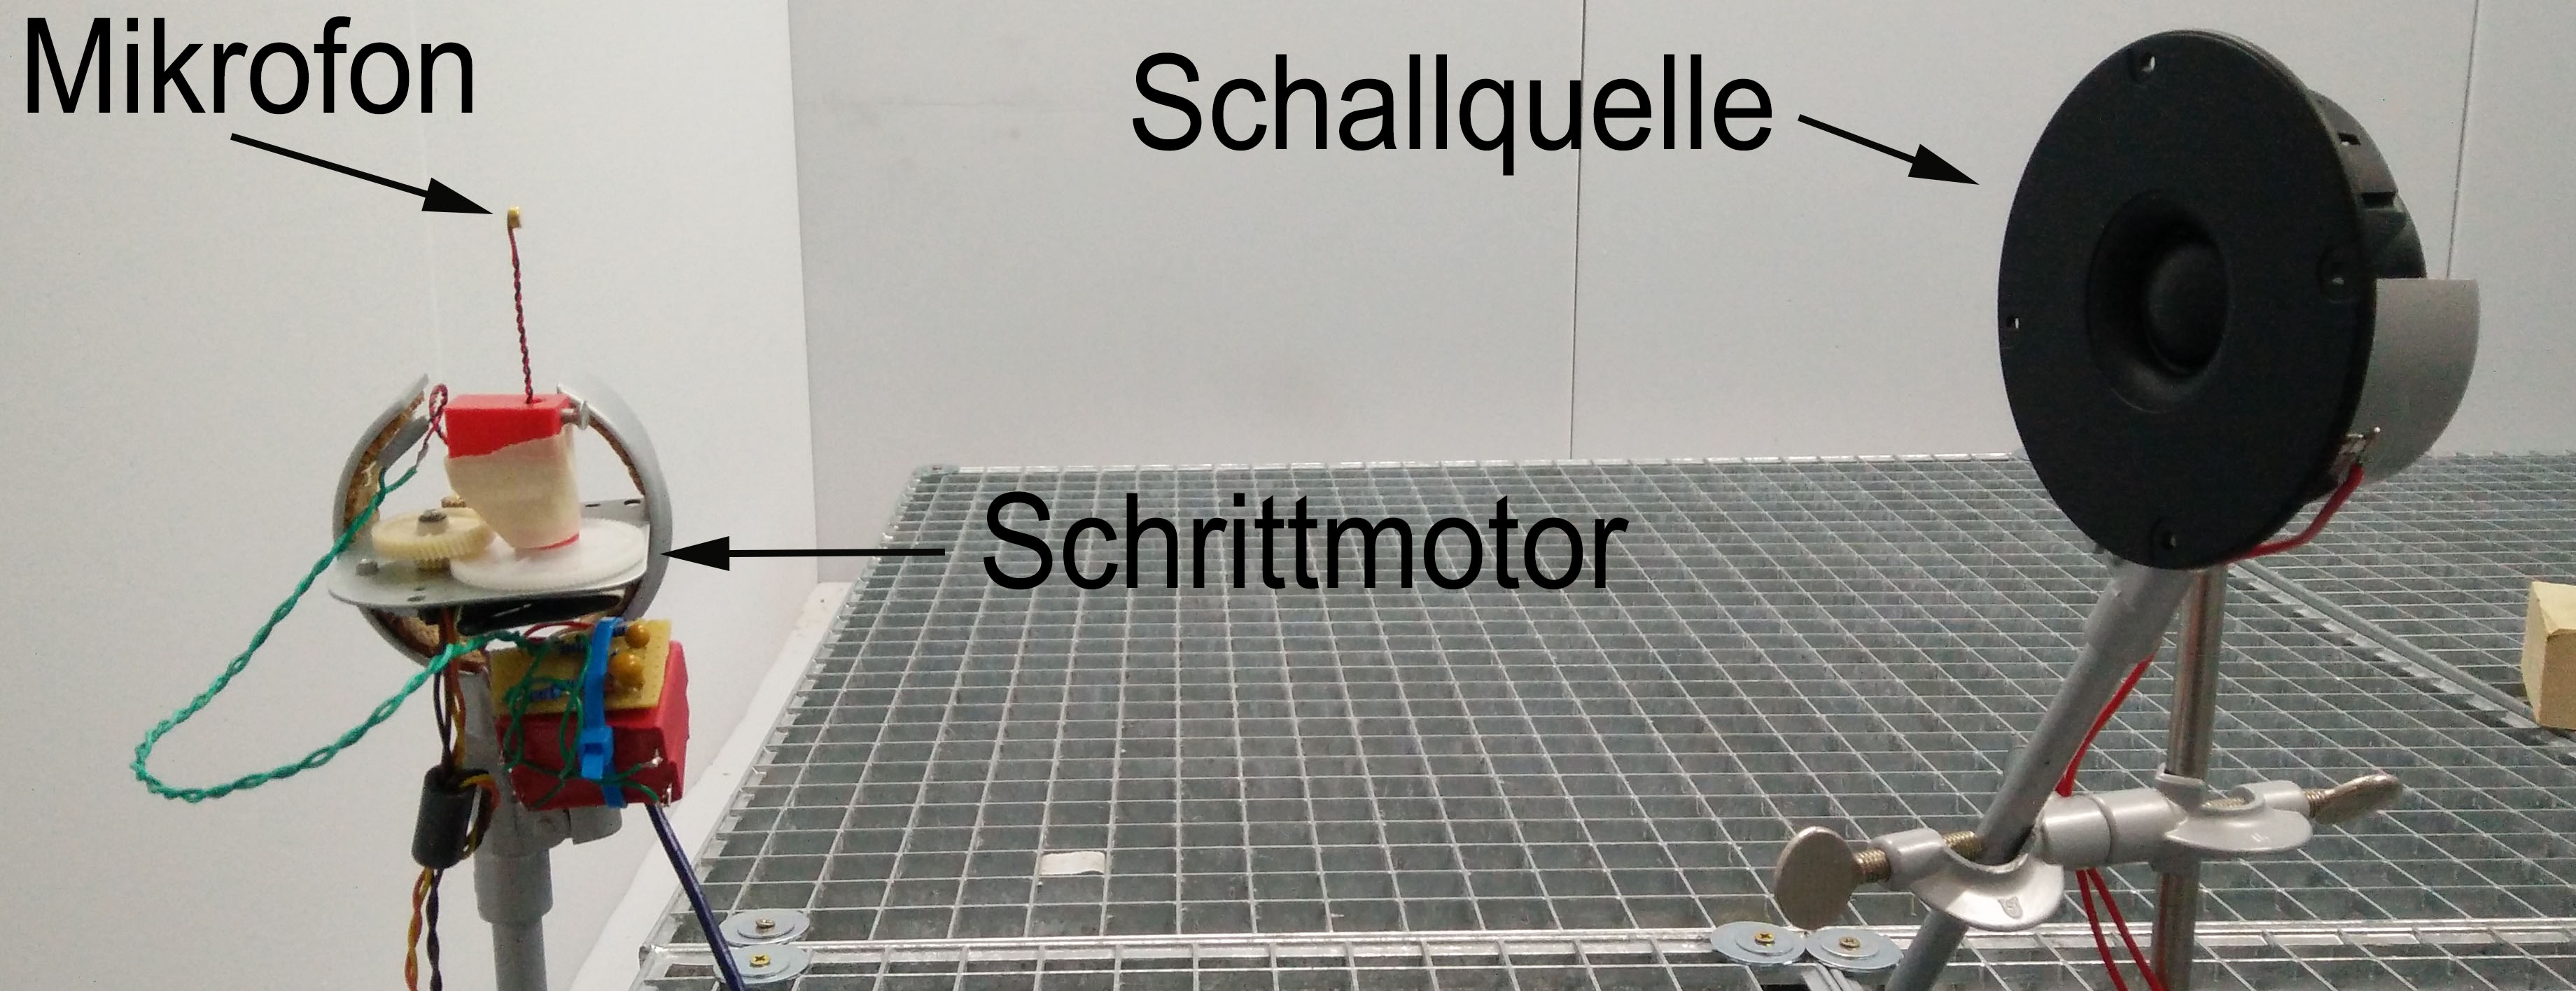
\includegraphics[width=0.8\linewidth]{img/chara_mess}
  \caption{Unsere Messapparatur für die Charakteristik eines Mikrofons}
\end{figure}
Die so ermittelten Daten können nun mittels des freien Plottingprogramms \textit{gnuplot}~\cite{Gnuplot} visualisiert werden, um die Richtcharakteristik abzulesen.
\begin{figure}[H]
  \centering
  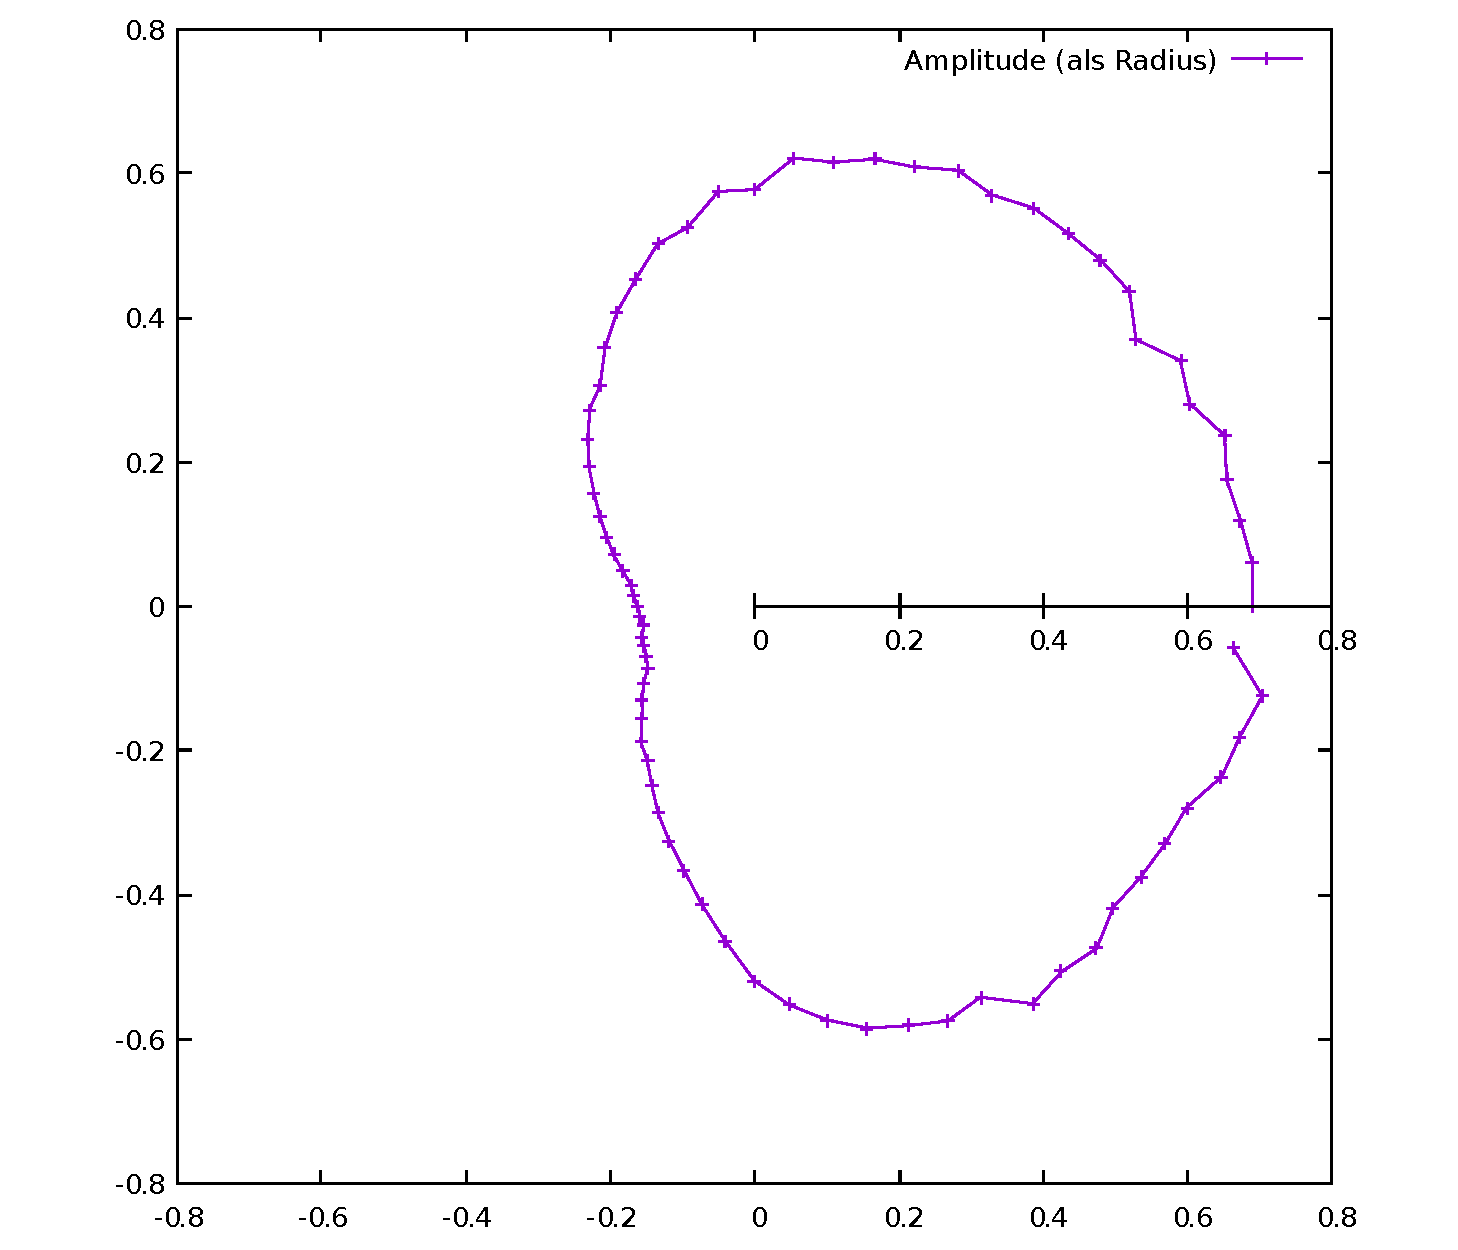
\includegraphics[width=0.45\linewidth]{img/badMic}
  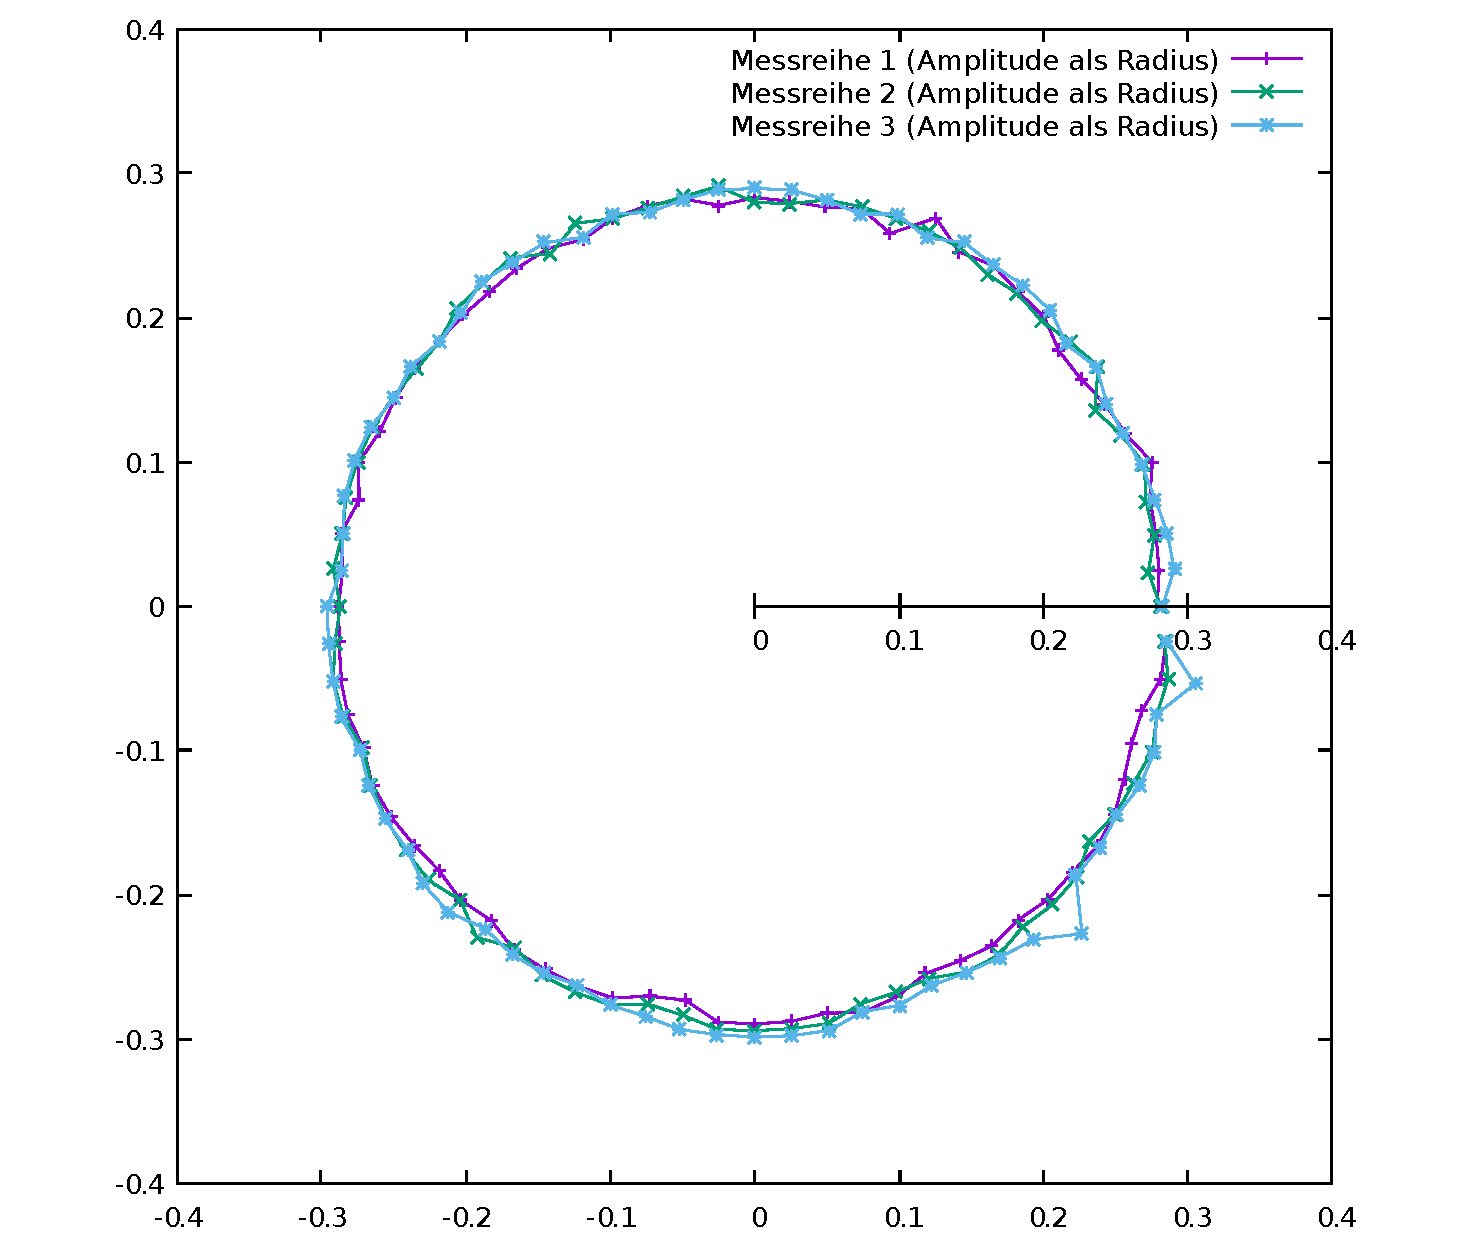
\includegraphics[width=0.45\linewidth]{img/goodMic}
  \caption{Auf den beiden Grafiken ist die gemessene Amplitude des Mikrofons über den Winkel aufgetragen. Bei der linken Grafik kann man feststellen, dass das vermessene Mikrofon eine sehr ungleichmäßige Charakteristik aufweist, diese Mikrofone haben wir zu Anfang verwendet. Auf der rechten Seite ist die Charakteristik der Mikrofone zu sehen, die wir in unserem aktuellen Testaufbau verwenden. Diese ist sehr gleichmäßig, weshalb wir die zuerst verwendeten Mikrofone durch diese Mikrofone ausgetauscht haben.}\label{fig:caracter}
\end{figure}
Für die reale Messapparatur haben wir vier Mikrofone in einem Tetraeder angeordnet. Dadurch, dass ein Tetraeder symmetrisch ist, sind die Fehler in alle Richtungen ungefähr gleich groß und die Richtungsbestimmung ist in allen Richtungen gleich gut. Um die Charakteristik der Mikrofone möglichst wenig zu verändern, haben wir die Mikrofone nur an ihrem Kabel mit dem Tetraeder verbunden. Dadurch ist der Schallschatten durch den Tetraeder relativ gering. Das Mittelstück des Tetraeders haben wir mit Hilfe eines 3D Druckers hergestellt.
\subsubsection{Audiointerface}
Auch an das Audiointerface, also die Verbindung von Mikrofonen zum Computer, gibt es bestimmte Voraussetzungen. So benötigt unser Verfahren mindestens 4 Mikrofone, jedoch lässt es sich einfach auf mehr Kanäle erweitern, was der Genauigkeit zugute kommt. Daher wird ein Audiointerface mit möglichst vielen Kanälen gesucht. Eine weitere wichtige Anforderung an das Audiointerface ist eine hohe Auflösung, da hierdurch die Signalqualität verbessert wird und digitale Verstärkung bei ausreichender Audioqualität möglich ist. Um die Elekretmikrofonkapseln an das Audiointerface anzuschließen, benötigt man zusätzlich eine Schaltung, welche das unsymmetrische Signal der Elektretmikrofonkapsel in ein symmetrisches Signal für das Audiointerface umwandelt. Außerdem muss diese die Phantomspeisung, die das Audiointerface bereitstellt und eine Spannung von 48V hat, in eine Tonaderspeisung für das Mikrofon konvertieren. Hierfür kommt die Schaltung von \cite{Powering_microphones} zum Einsatz.

\subsubsection{Software}
Um die echten Mikrofone für die Richtungsbestimmung zu verwenden, muss noch eine Verbindung zwischen dem Audiointerface und dem nächsten Modul geschaffen werden. Durch unseren modularen Aufbau lässt sich dies leicht implementieren. Wir haben dazu ein Programm in Java entwickelt, dass fähig ist, mehrkanalige Audiosignale in Echtzeit aufzunehmen und über TCP/IP an die Fourier-Transformation weiterzuleiten. Zur Umsetzung haben wir die Programmbibliothek \textit{portaudio} \cite{portaudio} verwendet. Diese Programmbibliothek hat den Vorteil, dass mehrere Audiokanäle zeitsynchronisiert eingelesen werden können, was sehr wichtig ist, damit unser Verfahren zur Richtungsbestimmung, welches auf der relativen Phasenlage basiert, funktioniert. \textit{Portaudio} wurde unter Java über das Java Native Interface (JNI) benutzt.

\subsection{Fourier-Transformation (Modul 2)}
Dieses Modul teilt die Audio-Signale in einzelnen Sinuswellen und bestimmt deren Phase und Amplitude. Um dies zu bewerkstelligen, lässt sich eine diskrete Fourier-Transformation verwenden. Die diskrete Fourier-Transformation bestimmt aus einem zeitdiskretem Signal die einzelnen Sinusschwingungen mit ihrer zugehörigen Phase und Amplitude, die zusammen das Signal bilden. Ein schneller Algorithmus um die diskrete Fourier-Transformation eines Signals zu berechnen ist die Fast Fourier-Transformation (FFT). Dieser ist schnell genug, um eine Echtzeitverarbeitung des Signals zu ermöglichen. Als Implementation der FFT haben wir \textit{FFTW}\cite{FFTW} verwendet, da \textit{FFTW} kostenlos, opensource und vergleichsweise schnell ist.
Das Fourier-Transformations Modul wurde aus Performancegründen in \textit{C++} implementiert.
Aus einer diskreten Fourier-Transformation von $n$ reellen Zahlen erhält man eine Liste aus $n$ komplexen Zahlen. Eine komplexe Zahl $z$ an der Stelle $i$ enthält die Amplituden- und Phaseninformation für die Frequenz $f$:
$$
f = \frac{i\cdot r}{n}
$$
$r$ ist dabei die Abtastrate des Signals. Die Amplitude $A$ des Sinus lässt sich mit dem Betrag der komplexen Zahl berechnen und die Phase $\phi$ mit dem Arcus-Tangens, dies entspricht der Koordinatentransformation von einem kartesischem in das polare Koordinatensystem:\\
\begin{minipage}{0.49\textwidth}
  $$
  A = \sqrt[]{{\Re(z)}^2 + {\Im(z)}^2}
  $$
  $$
  \phi = \operatorname{atan2}(\Im(z), \Re(z))
  $$
  $$
  \operatorname{atan2}(y,x) := \begin{cases} \arctan\frac{y}{x} & \mathrm{f\ddot ur}\ x > 0\\ \arctan\frac{y}{x} + \pi & \mathrm{f\ddot ur}\ x < 0,\ y \geq 0\\ \arctan\frac{y}{x} - \pi & \mathrm{f\ddot ur}\ x < 0,\ y < 0\\ +\pi/2 & \mathrm{f\ddot ur}\ x = 0,\ y > 0\\ -\pi/2 & \mathrm{f\ddot ur}\ x = 0,\ y < 0\\ 0 & \mathrm{f\ddot ur}\ x = 0,\ y = 0 \end{cases}
  $$
\end{minipage}
\begin{minipage}{0.49\textwidth}
  \begin{figure}[H]
    \centering
    \scalebox{.7}{% GNUPLOT: LaTeX picture with Postscript
\begingroup
  \fontfamily{phv}%
  \selectfont
\definecolor{t}{rgb}{0.5,0.5,0.5}
  \makeatletter
  \providecommand\color[2][]{%
    \GenericError{(gnuplot) \space\space\space\@spaces}{%
      Package color not loaded in conjunction with
      terminal option `colourtext'%
    }{See the gnuplot documentation for explanation.%
    }{Either use 'blacktext' in gnuplot or load the package
      color.sty in LaTeX.}%
    \renewcommand\color[2][]{}%
  }%
  \providecommand\includegraphics[2][]{%
    \GenericError{(gnuplot) \space\space\space\@spaces}{%
      Package graphicx or graphics not loaded%
    }{See the gnuplot documentation for explanation.%
    }{The gnuplot epslatex terminal needs graphicx.sty or graphics.sty.}%
    \renewcommand\includegraphics[2][]{}%
  }%
  \providecommand\rotatebox[2]{#2}%
  \@ifundefined{ifGPcolor}{%
    \newif\ifGPcolor
    \GPcolortrue
  }{}%
  \@ifundefined{ifGPblacktext}{%
    \newif\ifGPblacktext
    \GPblacktextfalse
  }{}%
  % define a \g@addto@macro without @ in the name:
  \let\gplgaddtomacro\g@addto@macro
  % define empty templates for all commands taking text:
  \gdef\gplbacktext{}%
  \gdef\gplfronttext{}%
  \makeatother
  \ifGPblacktext
    % no textcolor at all
    \def\colorrgb#1{}%
    \def\colorgray#1{}%
  \else
    % gray or color?
    \ifGPcolor
      \def\colorrgb#1{\color[rgb]{#1}}%
      \def\colorgray#1{\color[gray]{#1}}%
      \expandafter\def\csname LTw\endcsname{\color{white}}%
      \expandafter\def\csname LTb\endcsname{\color{black}}%
      \expandafter\def\csname LTa\endcsname{\color{black}}%
      \expandafter\def\csname LT0\endcsname{\color[rgb]{1,0,0}}%
      \expandafter\def\csname LT1\endcsname{\color[rgb]{0,1,0}}%
      \expandafter\def\csname LT2\endcsname{\color[rgb]{0,0,1}}%
      \expandafter\def\csname LT3\endcsname{\color[rgb]{1,0,1}}%
      \expandafter\def\csname LT4\endcsname{\color[rgb]{0,1,1}}%
      \expandafter\def\csname LT5\endcsname{\color[rgb]{1,1,0}}%
      \expandafter\def\csname LT6\endcsname{\color[rgb]{0,0,0}}%
      \expandafter\def\csname LT7\endcsname{\color[rgb]{1,0.3,0}}%
      \expandafter\def\csname LT8\endcsname{\color[rgb]{0.5,0.5,0.5}}%
    \else
      % gray
      \def\colorrgb#1{\color{black}}%
      \def\colorgray#1{\color[gray]{#1}}%
      \expandafter\def\csname LTw\endcsname{\color{white}}%
      \expandafter\def\csname LTb\endcsname{\color{black}}%
      \expandafter\def\csname LTa\endcsname{\color{black}}%
      \expandafter\def\csname LT0\endcsname{\color{black}}%
      \expandafter\def\csname LT1\endcsname{\color{black}}%
      \expandafter\def\csname LT2\endcsname{\color{black}}%
      \expandafter\def\csname LT3\endcsname{\color{black}}%
      \expandafter\def\csname LT4\endcsname{\color{black}}%
      \expandafter\def\csname LT5\endcsname{\color{black}}%
      \expandafter\def\csname LT6\endcsname{\color{black}}%
      \expandafter\def\csname LT7\endcsname{\color{black}}%
      \expandafter\def\csname LT8\endcsname{\color{black}}%
    \fi
  \fi
    \setlength{\unitlength}{0.0500bp}%
    \ifx\gptboxheight\undefined%
      \newlength{\gptboxheight}%
      \newlength{\gptboxwidth}%
      \newsavebox{\gptboxtext}%
    \fi%
    \setlength{\fboxrule}{0.5pt}%
    \setlength{\fboxsep}{1pt}%
\begin{picture}(5896.00,3600.00)%
    \gplgaddtomacro\gplbacktext{%
      \colorrgb{0.50,0.50,0.50}%
      \put(990,576){\makebox(0,0)[r]{\strut{}\color{t}$-1$}}%
      \colorrgb{0.50,0.50,0.50}%
      \put(990,1278){\makebox(0,0)[r]{\strut{}\color{t}$-0.5$}}%
      \colorrgb{0.50,0.50,0.50}%
      \put(990,1980){\makebox(0,0)[r]{\strut{}\color{t}$0$}}%
      \colorrgb{0.50,0.50,0.50}%
      \put(990,2681){\makebox(0,0)[r]{\strut{}\color{t}$0.5$}}%
      \colorrgb{0.50,0.50,0.50}%
      \put(990,3383){\makebox(0,0)[r]{\strut{}\color{t}$1$}}%
      \colorrgb{0.50,0.50,0.50}%
      \put(1098,396){\makebox(0,0){\strut{}\color{t}$-1$}}%
      \colorrgb{0.50,0.50,0.50}%
      \put(2216,396){\makebox(0,0){\strut{}\color{t}$-0.5$}}%
      \colorrgb{0.50,0.50,0.50}%
      \put(3335,396){\makebox(0,0){\strut{}\color{t}$0$}}%
      \colorrgb{0.50,0.50,0.50}%
      \put(4453,396){\makebox(0,0){\strut{}\color{t}$0.5$}}%
      \colorrgb{0.50,0.50,0.50}%
      \put(5571,396){\makebox(0,0){\strut{}\color{t}$1$}}%
      \csname LTb\endcsname%
      \put(3178,2050){\makebox(0,0)[l]{\strut{}$\phi$}}%
      \put(4341,1442){\makebox(0,0)[l]{\strut{}$A$}}%
    }%
    \gplgaddtomacro\gplfronttext{%
      \csname LTb\endcsname%
      \put(144,1979){\rotatebox{-270}{\makebox(0,0){\strut{}Imaginärteil}}}%
      \put(3334,126){\makebox(0,0){\strut{}Realteil}}%
      \csname LTb\endcsname%
      \put(4752,3230){\makebox(0,0)[r]{\strut{}z}}%
    }%
    \gplbacktext
    \put(0,0){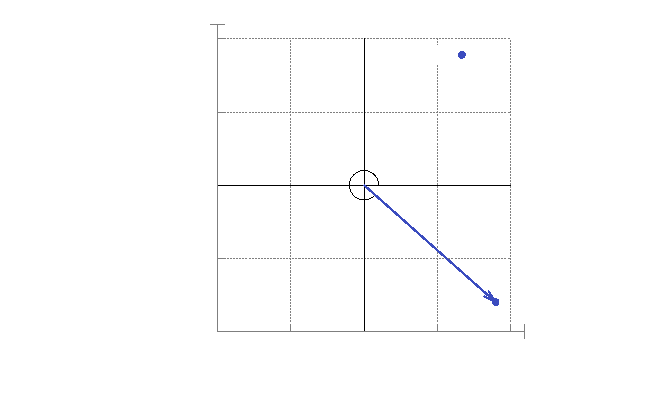
\includegraphics{img/polarconvert}}%
    \gplfronttext
  \end{picture}%
\endgroup
}
    \caption{Transformation von kartesischen zu polaren Koordinatensystem}
    \label{fig:polarconvert}
  \end{figure}
\end{minipage}
\vspace{20pt}
\\
Die Verwendung von $\operatorname{atan2}(y,x)$ anstelle von $\arctan\frac{y}{x}$ sorgt dafür, dass der richtige Winkel berechnet wird. $\arctan\frac{y}{x}$ liefert nur Winkel von -90\degree bis 90\degree, deswegen muss anhand des Vorzeichens von $x$ und $y$ bestimmt werden, in welchem Quadranten der Punkt liegt und der von $\arctan\frac{y}{x}$ gelieferte Winkel dementsprechend verschoben werden.

Das in Frequenz, Phase und Amplitude konvertierte Ergebnis der Fourier-Transformation wird dann gefiltert. Alle Frequenzen mit einer Amplitude, die kleiner als eine bestimmte Untergrenze ist, werden verworfen. Die verbleibenden Frequenzen werden an das Richtungsmodul übermittelt.

\subsection{Richtungsmodul (Modul 3)}
Die von der Fourier-Transformation bestimmten Tripel aus Frequenz, Phase und Amplitude werden vom Richtungsmodul weiter verarbeitet. In das Richtungsmodul können verschiedene Methoden der Richtungsbestimmung eingesetzt werden. Das Verfahren zur Richtungsbestimmung, das von dem Richtungsmodul verwendet wird, kann einfach ausgetauscht werden. Die ermittelten Richtungen werden an die Ausgabe weitergesendet um sie dort auszugeben oder zur Filterung des Audio-Signals zu verwenden.
Das Richtungsmodul ist in C++ geschrieben und verwendet \textit{LAPACK}\cite{Anderson:1990:LPL:110382.110385}.
\subsection{Ausgabemodul (Modul 4)}
\begin{wrapfigure}{r}{0.5\textwidth}
	\centering
	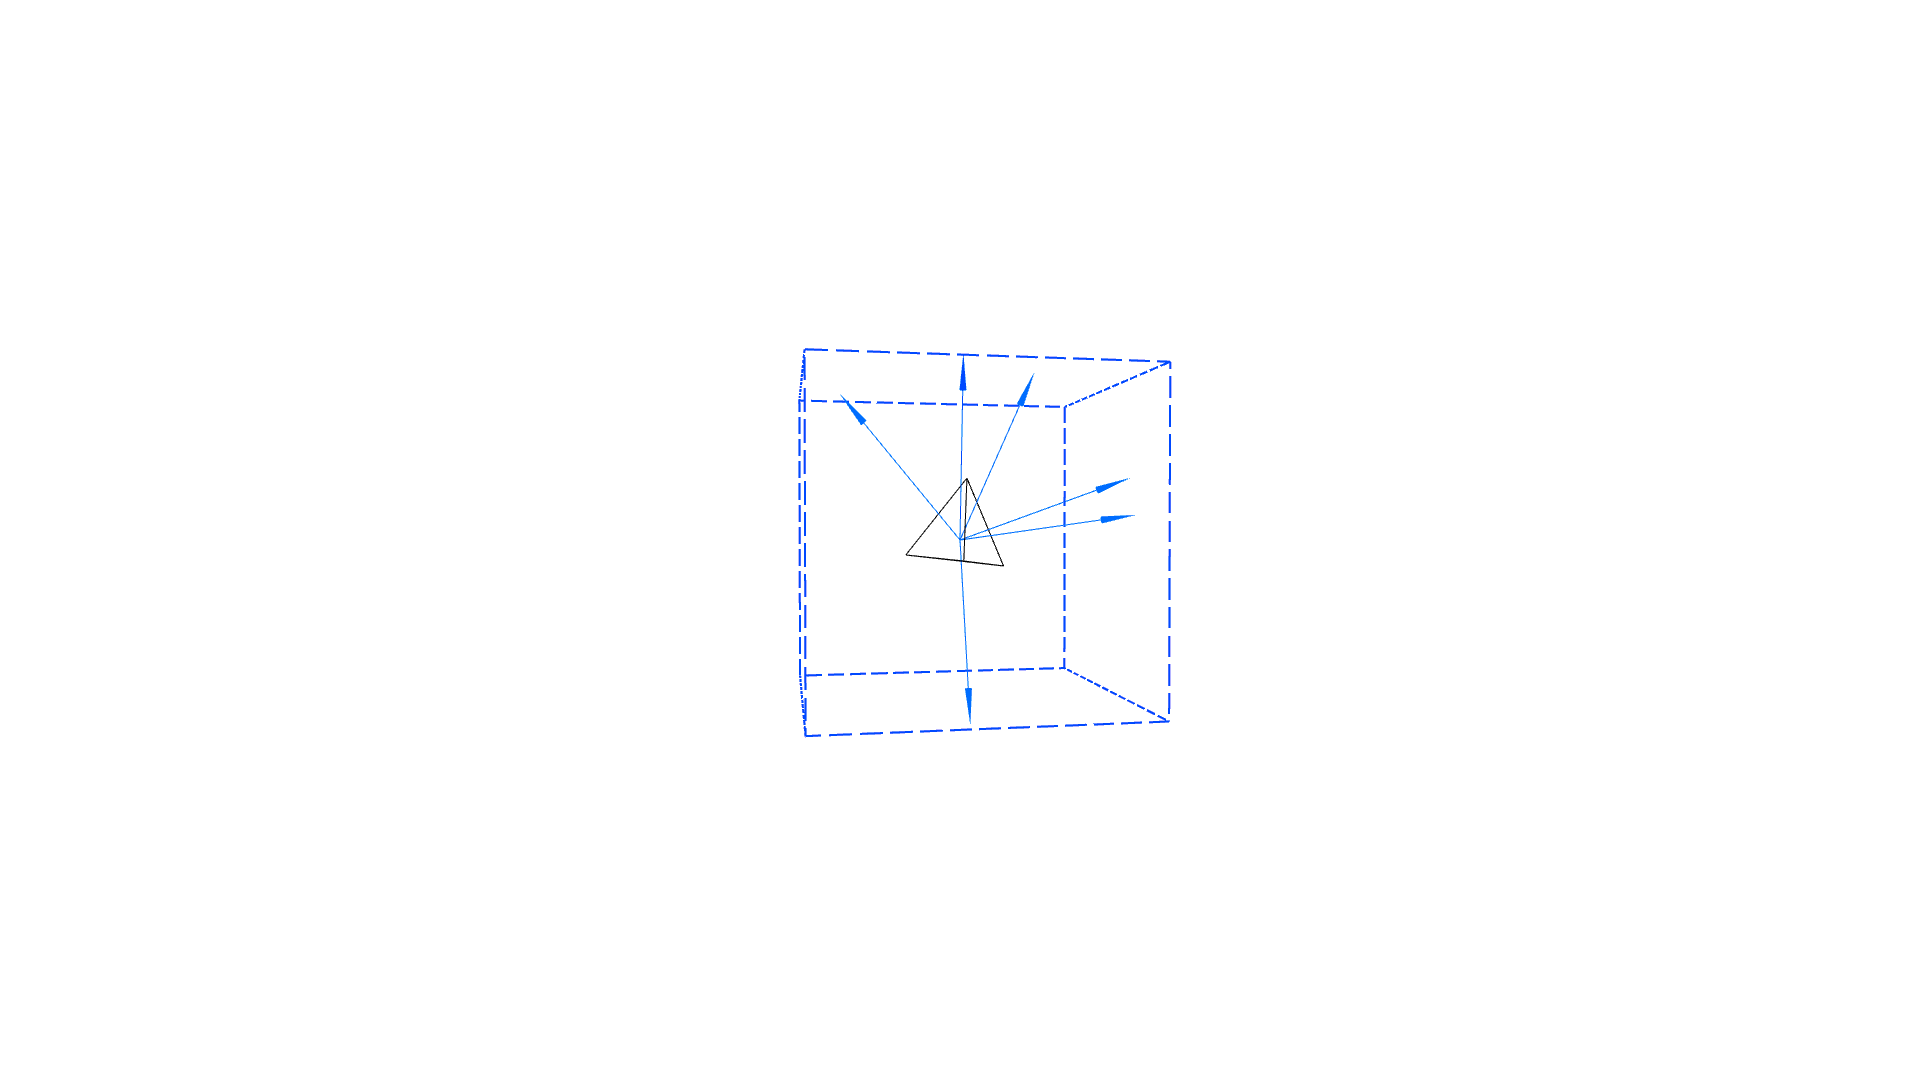
\includegraphics[width=0.49\textwidth]{img/output}
	\caption{Screenshot unseres Beispiel-Ausgabemoduls}
	\label{fig:output}
\end{wrapfigure}
Wir haben ein Beispiel-Ausgabemodul in Javascript implementiert. Mit diesem ist es möglich, die Positionsdaten zu visualisieren, was das unmittelbare Evaluieren stark vereinfacht. Die Programmiersprache Javascript haben wir gewählt, damit dieses Ausgabemodul auf jedem Endgerät mit modernem Webbrowser, wie z.B. Smartphones oder Laptops, ausgeführt werden kann.\\
Die Simulation enthält eine weitere Implementation eines Ausgabemoduls. Auch diese visualisiert die bestimmten Richtungen, erlaubt es aber, diese auf der gleichen Benutzeroberfläche wie die Sollrichtung anzuzeigen. Dies gibt ein sehr direktes Feedback beim Entwickeln des Algorithmus zur Richtungsbestimmung. Dieses letzte Modul könnte allerdings, dank unseres modularen Konzeptes, bei Bedarf auch anders, z.B. als Plugin für eine \textit{Digital Audio Workstation} (\textit{DAW}) implementiert werden.
\subsection{Testen der einzelnen Module}
Ein weiterer Vorteil der Modularität ist, dass jedes Modul unabhängig von den anderen Modulen funktionsfähig ist. Dadurch kann die korrekte Funktionsweise für jedes Modul einzeln überprüft werden und man kann Fehler besser lokalisieren.
Die Audiosimulation haben wir mithilfe eines selbstgeschriebenem Plotting Programms überprüft. Dieses stellt die von der Audiosimulation versendeten Samples in Abhängigkeit der Zeit dar. Damit kann manuell die Phasendifferenz von dem Graphen abgelesen und mit dem erwarteten Wert verglichen werden.
\begin{figure} [H]
	\centering
  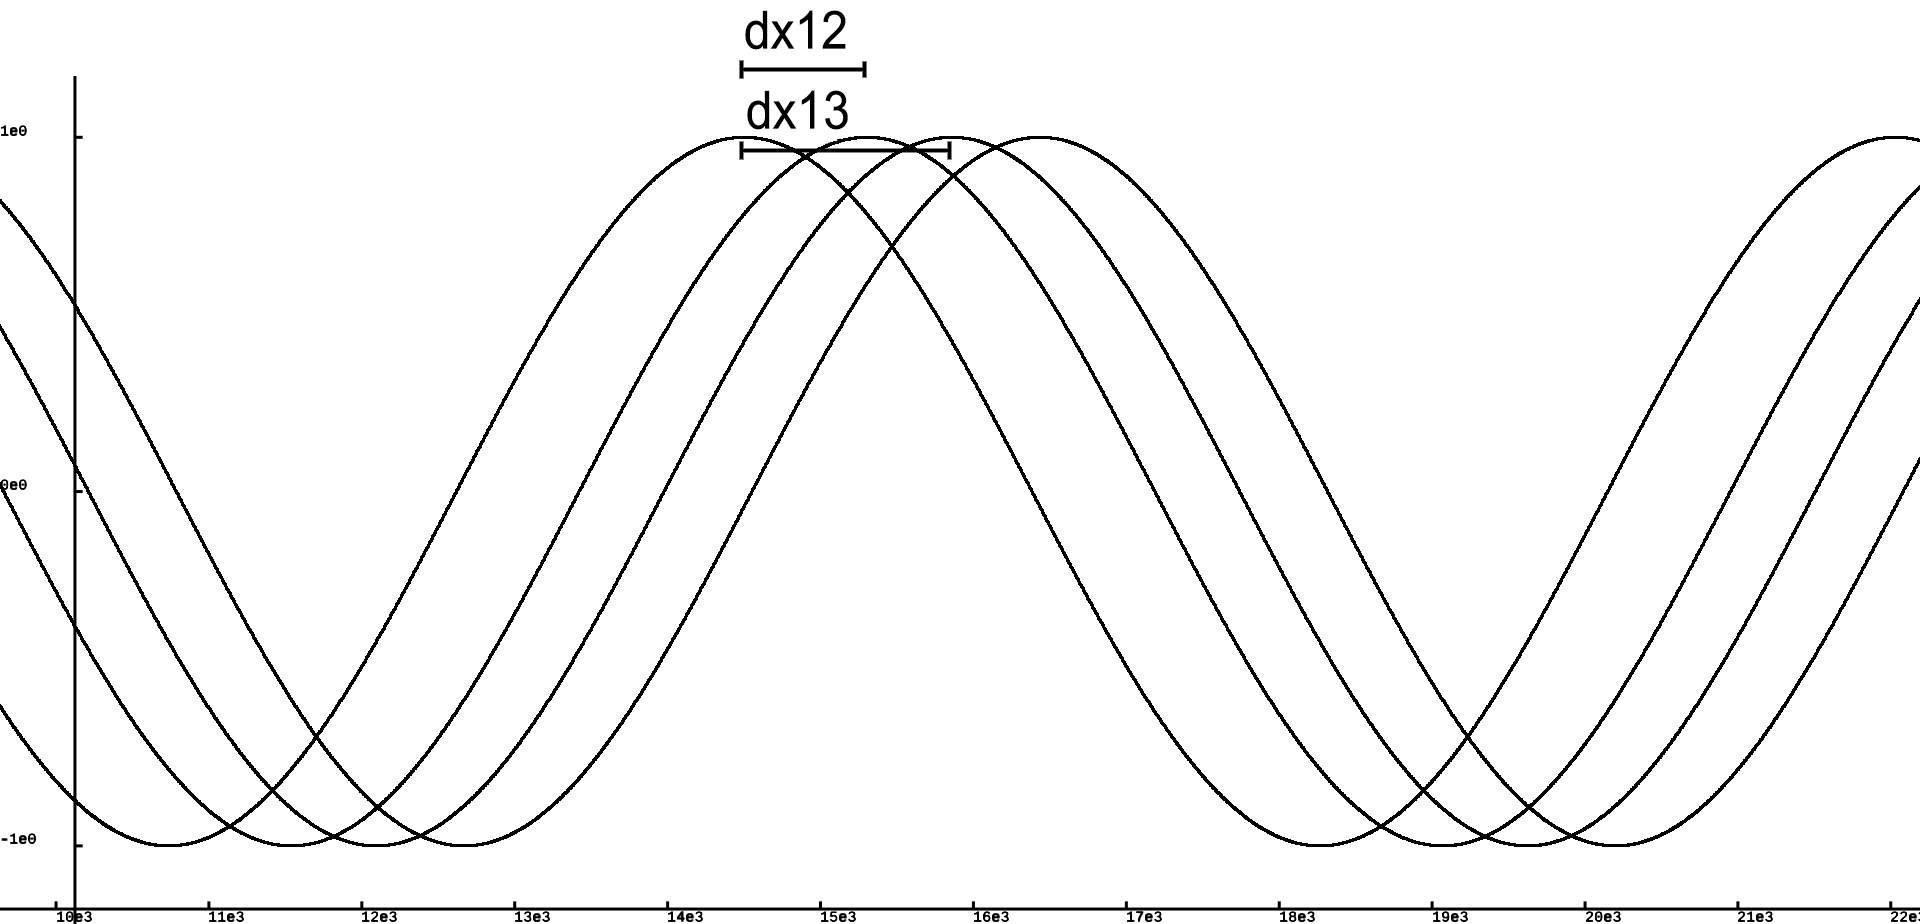
\includegraphics[width=.8\linewidth]{img/glplot}
  \caption{Screenshot unseres Plotting Programms}
  \label{fig:glplot}
\end{figure}

Die Fourier-Transformation konnten wir mit der vorher überprüften Audiosimulation testen. Dazu haben wir die von der Fourier-Transformation bestimmten Frequenz, Phase und Amplitude Tripel mit den tatsächlich in der Simulation eingestellten Werten verglichen.
Durch das Testen der einzelnen Module konnten wir effizient die vorhandenen Fehler, wie die falsche Berechnung der Phase und einen Fehler in der Distanzberechnung der Audiosimulation, finden und beheben.

    \section{Eindimensionale Richtungsbestimmung} \todo{Durchlesen + überprüfen}
  Um den Algorithmus, der aus den Phasendifferenzen die Richtung zurückrechnet zu entwickeln haben wir mit der
einfachsten Stufe der Richtungsbestimmung, der eindimensionale Richtungsbestimmung, angefangen:
\begin{figure}[H]
  \centering
  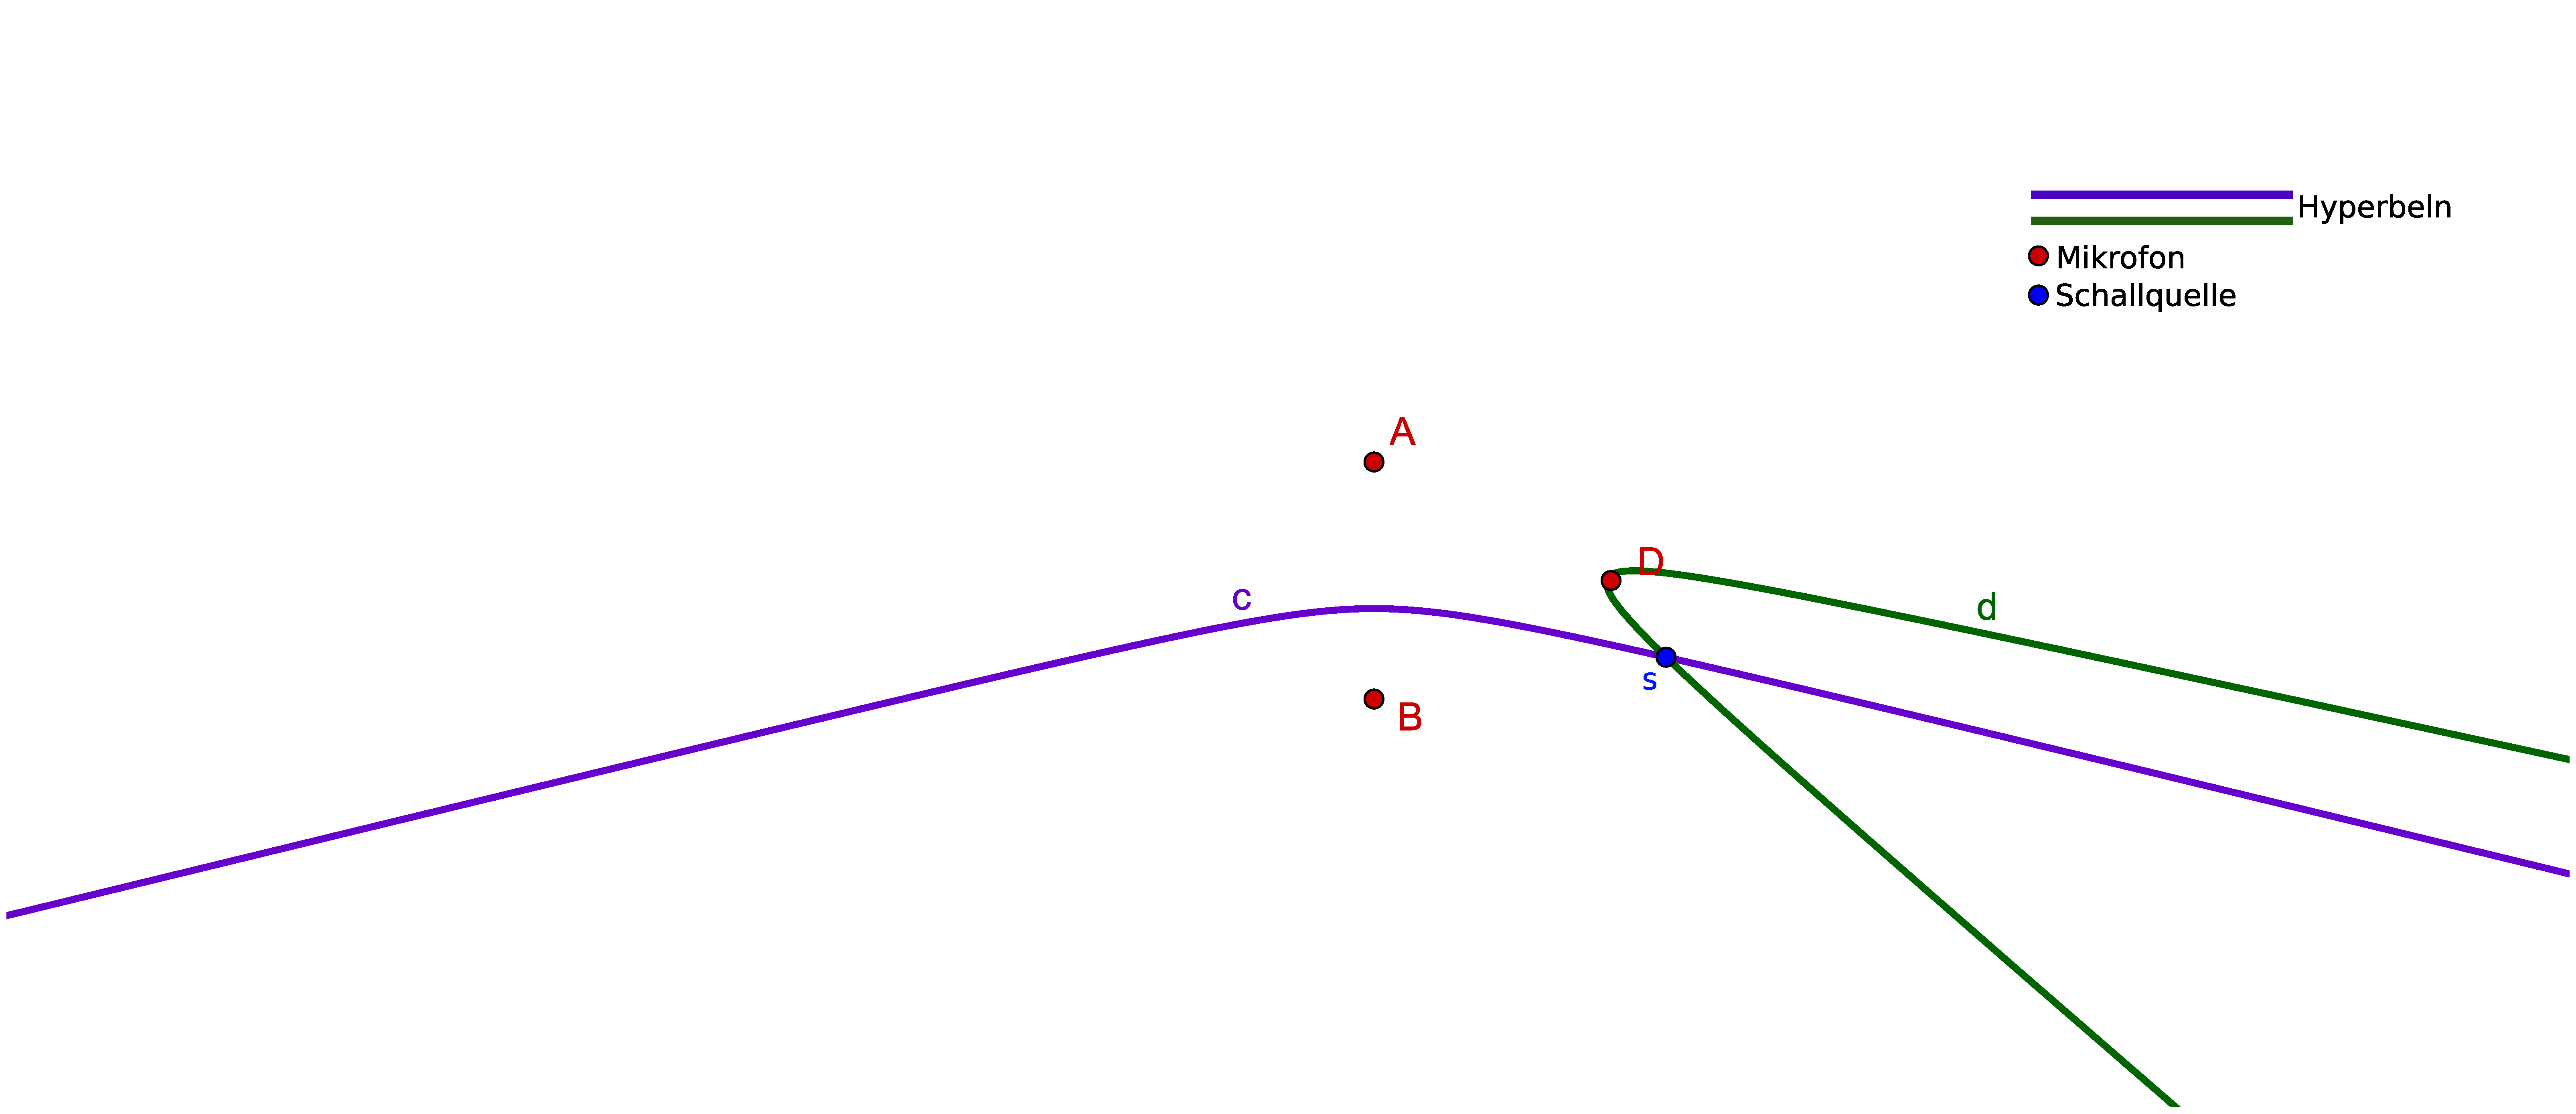
\includegraphics[width=\linewidth]{img/skizze1d}
  \caption{Skizze einer eindimensionalen Richtungsbestimmung}
\label{fig:skizz1d}
\end{figure}

In Abbildung~\ref{fig:skizz1d} sieht man zwei Mikrofone $M_1$ und $M_2$, die den Schall der Schallquelle $S$ aufnehmen. Dadurch, dass $M_2$ weiter von der Schallquelle entfernt ist als $M_1$ braucht der Schall länger um $M_2$ zu erreichen. Wenn man die von den Mikrofonen aufgenommenen Schallwellen vergleicht sieht man dies in Form des rot markierten Gangunterschieds:
\begin{figure}[H]
% GNUPLOT: LaTeX picture with Postscript
\begingroup
  \fontfamily{phv}%
  \selectfont
\definecolor{t}{rgb}{0.5,0.5,0.5}
  \makeatletter
  \providecommand\color[2][]{%
    \GenericError{(gnuplot) \space\space\space\@spaces}{%
      Package color not loaded in conjunction with
      terminal option `colourtext'%
    }{See the gnuplot documentation for explanation.%
    }{Either use 'blacktext' in gnuplot or load the package
      color.sty in LaTeX.}%
    \renewcommand\color[2][]{}%
  }%
  \providecommand\includegraphics[2][]{%
    \GenericError{(gnuplot) \space\space\space\@spaces}{%
      Package graphicx or graphics not loaded%
    }{See the gnuplot documentation for explanation.%
    }{The gnuplot epslatex terminal needs graphicx.sty or graphics.sty.}%
    \renewcommand\includegraphics[2][]{}%
  }%
  \providecommand\rotatebox[2]{#2}%
  \@ifundefined{ifGPcolor}{%
    \newif\ifGPcolor
    \GPcolortrue
  }{}%
  \@ifundefined{ifGPblacktext}{%
    \newif\ifGPblacktext
    \GPblacktextfalse
  }{}%
  % define a \g@addto@macro without @ in the name:
  \let\gplgaddtomacro\g@addto@macro
  % define empty templates for all commands taking text:
  \gdef\gplbacktext{}%
  \gdef\gplfronttext{}%
  \makeatother
  \ifGPblacktext
    % no textcolor at all
    \def\colorrgb#1{}%
    \def\colorgray#1{}%
  \else
    % gray or color?
    \ifGPcolor
      \def\colorrgb#1{\color[rgb]{#1}}%
      \def\colorgray#1{\color[gray]{#1}}%
      \expandafter\def\csname LTw\endcsname{\color{white}}%
      \expandafter\def\csname LTb\endcsname{\color{black}}%
      \expandafter\def\csname LTa\endcsname{\color{black}}%
      \expandafter\def\csname LT0\endcsname{\color[rgb]{1,0,0}}%
      \expandafter\def\csname LT1\endcsname{\color[rgb]{0,1,0}}%
      \expandafter\def\csname LT2\endcsname{\color[rgb]{0,0,1}}%
      \expandafter\def\csname LT3\endcsname{\color[rgb]{1,0,1}}%
      \expandafter\def\csname LT4\endcsname{\color[rgb]{0,1,1}}%
      \expandafter\def\csname LT5\endcsname{\color[rgb]{1,1,0}}%
      \expandafter\def\csname LT6\endcsname{\color[rgb]{0,0,0}}%
      \expandafter\def\csname LT7\endcsname{\color[rgb]{1,0.3,0}}%
      \expandafter\def\csname LT8\endcsname{\color[rgb]{0.5,0.5,0.5}}%
    \else
      % gray
      \def\colorrgb#1{\color{black}}%
      \def\colorgray#1{\color[gray]{#1}}%
      \expandafter\def\csname LTw\endcsname{\color{white}}%
      \expandafter\def\csname LTb\endcsname{\color{black}}%
      \expandafter\def\csname LTa\endcsname{\color{black}}%
      \expandafter\def\csname LT0\endcsname{\color{black}}%
      \expandafter\def\csname LT1\endcsname{\color{black}}%
      \expandafter\def\csname LT2\endcsname{\color{black}}%
      \expandafter\def\csname LT3\endcsname{\color{black}}%
      \expandafter\def\csname LT4\endcsname{\color{black}}%
      \expandafter\def\csname LT5\endcsname{\color{black}}%
      \expandafter\def\csname LT6\endcsname{\color{black}}%
      \expandafter\def\csname LT7\endcsname{\color{black}}%
      \expandafter\def\csname LT8\endcsname{\color{black}}%
    \fi
  \fi
    \setlength{\unitlength}{0.0500bp}%
    \ifx\gptboxheight\undefined%
      \newlength{\gptboxheight}%
      \newlength{\gptboxwidth}%
      \newsavebox{\gptboxtext}%
    \fi%
    \setlength{\fboxrule}{0.5pt}%
    \setlength{\fboxsep}{1pt}%
\begin{picture}(8730.00,3600.00)%
    \gplgaddtomacro\gplbacktext{%
      \colorrgb{0.50,0.50,0.50}%
      \put(990,576){\makebox(0,0)[r]{\strut{}\color{t}$-1$}}%
      \colorrgb{0.50,0.50,0.50}%
      \put(990,857){\makebox(0,0)[r]{\strut{}\color{t}$-0.8$}}%
      \colorrgb{0.50,0.50,0.50}%
      \put(990,1137){\makebox(0,0)[r]{\strut{}\color{t}$-0.6$}}%
      \colorrgb{0.50,0.50,0.50}%
      \put(990,1418){\makebox(0,0)[r]{\strut{}\color{t}$-0.4$}}%
      \colorrgb{0.50,0.50,0.50}%
      \put(990,1699){\makebox(0,0)[r]{\strut{}\color{t}$-0.2$}}%
      \colorrgb{0.50,0.50,0.50}%
      \put(990,1980){\makebox(0,0)[r]{\strut{}\color{t}$0$}}%
      \colorrgb{0.50,0.50,0.50}%
      \put(990,2260){\makebox(0,0)[r]{\strut{}\color{t}$0.2$}}%
      \colorrgb{0.50,0.50,0.50}%
      \put(990,2541){\makebox(0,0)[r]{\strut{}\color{t}$0.4$}}%
      \colorrgb{0.50,0.50,0.50}%
      \put(990,2822){\makebox(0,0)[r]{\strut{}\color{t}$0.6$}}%
      \colorrgb{0.50,0.50,0.50}%
      \put(990,3102){\makebox(0,0)[r]{\strut{}\color{t}$0.8$}}%
      \colorrgb{0.50,0.50,0.50}%
      \put(990,3383){\makebox(0,0)[r]{\strut{}\color{t}$1$}}%
      \colorrgb{0.50,0.50,0.50}%
      \put(1098,396){\makebox(0,0){\strut{}\color{t}$0$}}%
      \colorrgb{0.50,0.50,0.50}%
      \put(1833,396){\makebox(0,0){\strut{}\color{t}$2$}}%
      \colorrgb{0.50,0.50,0.50}%
      \put(2569,396){\makebox(0,0){\strut{}\color{t}$4$}}%
      \colorrgb{0.50,0.50,0.50}%
      \put(3304,396){\makebox(0,0){\strut{}\color{t}$6$}}%
      \colorrgb{0.50,0.50,0.50}%
      \put(4040,396){\makebox(0,0){\strut{}\color{t}$8$}}%
      \colorrgb{0.50,0.50,0.50}%
      \put(4775,396){\makebox(0,0){\strut{}\color{t}$10$}}%
      \colorrgb{0.50,0.50,0.50}%
      \put(5511,396){\makebox(0,0){\strut{}\color{t}$12$}}%
      \colorrgb{0.50,0.50,0.50}%
      \put(6246,396){\makebox(0,0){\strut{}\color{t}$14$}}%
    }%
    \gplgaddtomacro\gplfronttext{%
      \csname LTb\endcsname%
      \put(144,1979){\rotatebox{-270}{\makebox(0,0){\strut{}Amplitude}}}%
      \put(3856,126){\makebox(0,0){\strut{}Zeit[t]}}%
      \csname LTb\endcsname%
      \put(7910,3293){\makebox(0,0)[r]{\strut{}Mikrofon 1}}%
      \csname LTb\endcsname%
      \put(7910,3113){\makebox(0,0)[r]{\strut{}Mikrofon 2}}%
      \csname LTb\endcsname%
      \put(1098,1839){\makebox(0,0)[l]{\strut{}Gangunterschied}}%
    }%
    \gplbacktext
    \put(0,0){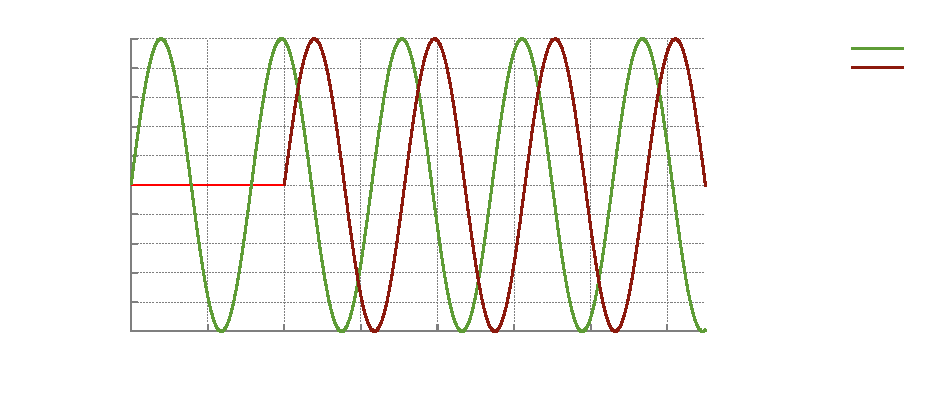
\includegraphics{img/welle1d}}%
    \gplfronttext
  \end{picture}%
\endgroup

\caption{Vergleich der von den beiden Mikrofonen aufgenommenen Wellen}
\label{fig:welle1d}
\end{figure}
Wir können von den von den Mikrofonen aufgenommenen Wellen nur die Phasenverschiebung bestimmen. Deswegen können wir den Gangunterschied nicht direkt bestimmen, er setzt sich aus einer unbekannten Anzahl von kompletten Schwingungen und der Differenz der Phasenverschiebungen zusammen. Man erhält für die Differenz der Abstände einer Schallquelle $S$ von zwei Mikrofonen $M_1$ und $M_2$ mit der gemessenen Phase $\phi_1$ und $\phi_2$: $$n\ + \Delta{x_{12}}$$ $\lambda$ ist hierbei die Wellenlänge, $n$ die unbekannte Anzahl an Schwingungen und $\Delta{x_{12}}$ der Gangunterschied, dem man aus dem Phasenunterschied bestimmen kann:
$$\Delta{x_{ij}} = \frac{c(\phi_i - \phi_j)}{{2\pi}f}\:\textrm{mit}\:i = 1\:\textrm{und}\:j = 2$$
$c$ ist die Schallgeschwindigkeit und $f$ die Frequenz des Schallwelle.
Jedes Mikrofon $M_i$ hat einen zugehörigen Ortsvektor $\vec{m}_i = \begin{pmatrix} m_{i_x} \\ m_{i_y}  \end{pmatrix}$, die Schallquelle hat den Ortsvektor $\vec{s} = \begin{pmatrix} {s_x} \\ {s_y}  \end{pmatrix}$. Der Abstand eines Mikrofons von der Schallquelle ist gegeben durch den Satz des Pythagoras:
$$\abs{\vec{m}_i - \vec{s}} = \sqrt{{(m_{i_x} - s_x)}^2 + {(m_{i_y} - s_y)}^2}$$
Damit erhält man für die Differenz der Abstände der Mikrofone die Gleichung
$$\abs{\vec{m}_1 - \vec{s}} - \abs{\vec{m}_2 - \vec{s}} = n\lambda + \Delta{x_{12}}$$
$$\sqrt{{(m_{1_x} - s_x)}^2 + {(m_{1_y} - s_y)}^2} - \sqrt{{(m_{2_x} - s_x)}^2 + {(m_{2_y} - s_y)}^2} = n\lambda + \Delta{x_{12}}$$$s_y$ ist konstant für alle möglichen Positionen der Schallquelle. Dadurch hat die Gleichung aber immer noch zwei Unbekannte, $s_x$ und $n$, und ist deswegen nicht eindeutig lösbar. Man kann eine eindeutig lösbare Gleichung erhalten, wenn der Abstand der Mikrofone maximal halb so groß wie die Wellenlänge ist. Dann macht die Welle maximal eine halbe Schwingung mehr zu einem Mikrofon als zu dem anderen und die unbekannte Anzahl an Schwingungen $n\lambda$ entfällt. Dann hat die Gleichung nur eine Unbekannte, $s_x$
$$\abs{\vec{m}_1 - \vec{s}} - \abs{\vec{m}_2 - \vec{s}} = \Delta{x_{12}}$$
$$\sqrt{{(m_{1_x} - s_x)}^2 + {(m_{1_y} - s_y)}^2} - \sqrt{{(m_{2_x} - s_x)}^2 + {(m_{2_y} - s_y)}^2} = \Delta{x_{12}}$$
Den dadurch bestimmten Ortvektor kann man dann in eine Gerade $g$ umwandeln, die der Richtung, in der sich die Schallquelle befindet, entspricht:
$$g: \vec{x} = r \cdot \vec{s}$$
Da eine eindimensionale Ortung sehr einfach und ohne großen Anwendungsbereich ist haben wir diesen Algorithmus anschließend auf zwei Dimensionen übertragen.

    \section{Zweidimensionale Richtungsbestimmung}
\subsection{Erweiterung der Theorie}
Um die eindimensionale Richtungsbestimmung auf zwei Dimensionen zu erweitern, muss man lediglich $s_y$ als nicht mehr konstant betrachten. Dadurch hat die Gleichung, die für das Eindimensionale eindeutig war, nun zwei Unbekannte: $s_x$ und $s_y$. Um im Zweidimensionalen eine Ortung durchzuführen, wird deswegen ein drittes Mikrofon $M_3$ benötigt. Auch der Abstand zwischen dem dritten Mikrofon und dem ersten darf maximal so groß wie die Wellenlänge sein. Mit dem dritten Mikrofon kann eine weitere Gleichung, die die Wegdifferenz zwischen dem ersten und dem dritten Mikrofon $\Delta{x_{13}}$ enthält, aufgestellt werden. Man erhält das Gleichungssystem:
\begin{gather}\begin{vmatrix}
  \abs{\vec{m}_1 - \vec{s}} - \abs{\vec{m}_2 - \vec{s}} = \Delta{x_{12}} \\
  \abs{\vec{m}_1 - \vec{s}} - \abs{\vec{m}_3 - \vec{s}} = \Delta{x_{13}}
\end{vmatrix}\\
\begin{vmatrix}
  \sqrt{{(m_{1x} - s_x)}^2 + {(m_{1y} - s_y)}^2} - \sqrt{{(m_{2x} - s_x)}^2 + {(m_{2y} - s_y)}^2} = \Delta{x_{12}} \\
  \sqrt{{(m_{1x} - s_x)}^2 + {(m_{1y} - s_y)}^2} - \sqrt{{(m_{3x} - s_x)}^2 + {(m_{3y} - s_y)}^2} = \Delta{x_{13}}
\end{vmatrix}
\end{gather}
Grafisch veranschaulicht entspricht dieses Gleichungssystem der Suche nach dem Schnittpunkt von zwei halben Hyperbeln um zwei der Mikrofone:
\begin{figure}[H]
	\vspace{-20pt}
  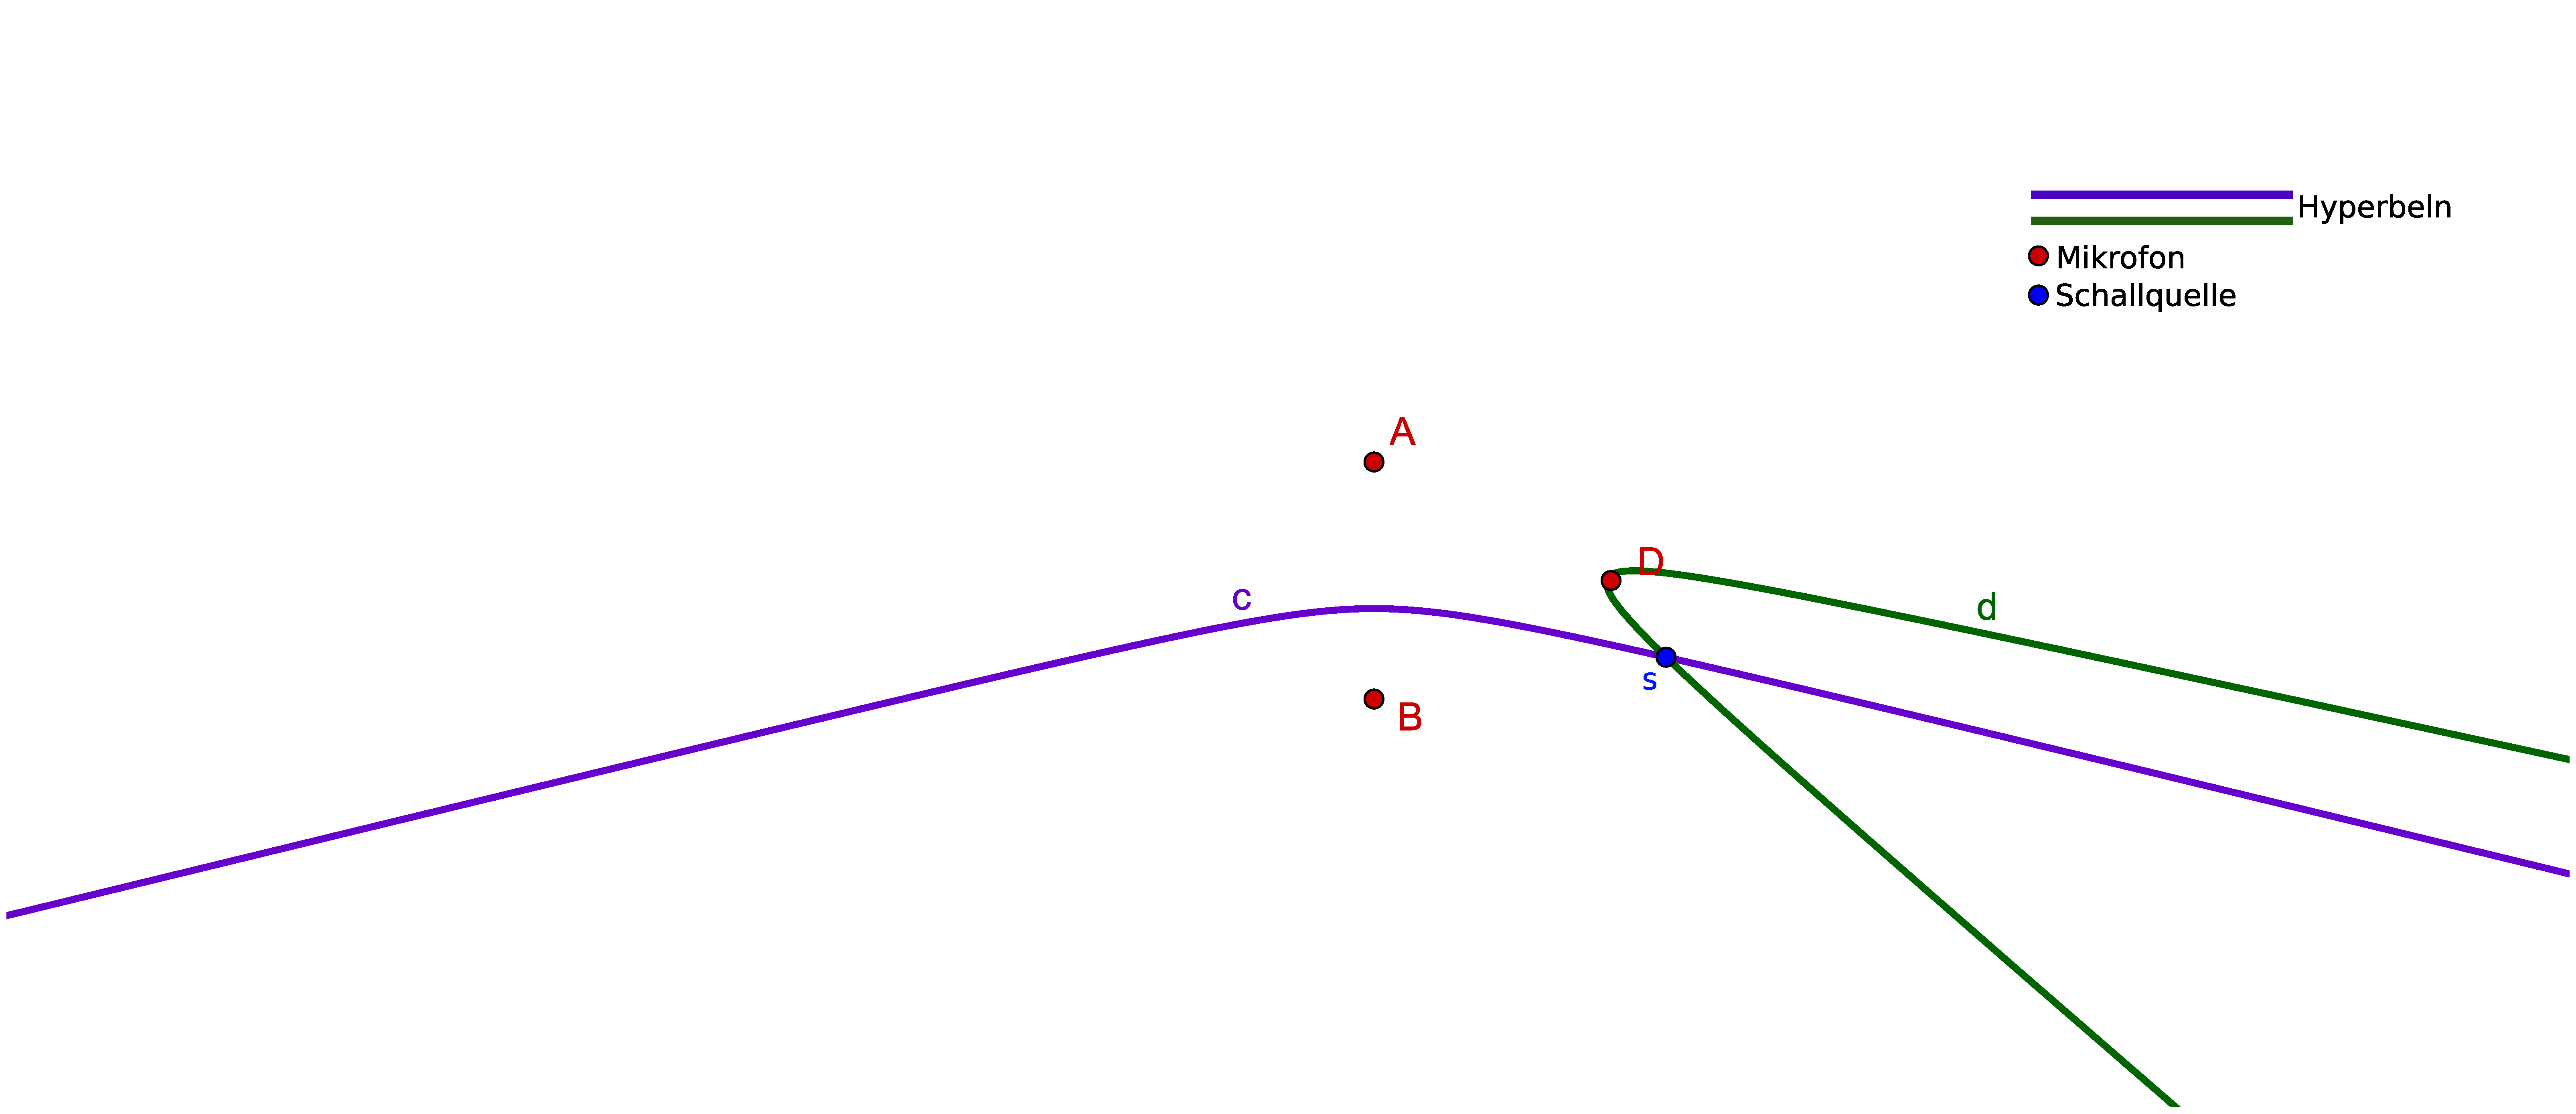
\includegraphics[width=\linewidth]{img/skizze1d}
  \caption{Veranschaulichung des Gleichungssystems durch den Schnittpunkt von zwei Hyperbeln. Die roten Punkte stellen die Mikrofone dar und der blaue Punkt die Schallquelle.}
\end{figure}

\subsection{Analytische Lösung des Gleichungssystems}
Dieses Gleichungssystem haben wir mithilfe des Computeralgebrasystems \textit{Wolfram Mathematica}~\cite{mathematica} nach $\vec{s}$ aufgelöst:
\begin{lstlisting}[language=Mathematica,caption={Befehl für das Lösen des Gleichungssystem in \textit{Mathematica}.}]
  Solve[{
    Sqrt[{(m1x - sx)}^2 + {(m1y - sy)}^2] - Sqrt[{(m2x - sx)}^2 + {(m2y - sy)}^2] = dx12,
    Sqrt[{(m1x - sx)}^2 + {(m1y - sy)}^2] - Sqrt[{(m3x - sx)}^2 + {(m3y - sy)}^2] = dx13},
  {sx, sy}]
\end{lstlisting}
Da das Gleichungssystem nicht linear ist, ist die Lösung sehr kompliziert, gedruckt entspricht sie fünf Seiten. \textit{Mathematica} findet für dieses Gleichungssystem außerdem zwei allgemeine reelle Lösungen, man erhält also zwei mögliche Richtungen.

    \section{Dreidimensionale Richtungsbestimmung}
\subsection{Erweiterung der Theorie}
Um die Richtungsbestimmung dann auf drei Dimensionen zu erweitern, müssen zuerst die Ortsvektoren der Mikrofone und der Schallquelle auf drei Dimensionen erweitert werden:
\begin{equation}
    \vec{m}_i = \begin{pmatrix}
        m_{ix} \\
        m_{iy} \\
        m_{iz}
    \end{pmatrix} \quad\quad
    \vec{s} = \begin{pmatrix}
        {s_x} \\
        {s_y} \\
        {s_z}
    \end{pmatrix}
\end{equation}
Mit den angepassten Ortsvektoren erhält man eine neue Formel für die Abstandsberechnung zwischen einem Mikrofon und der Schallquelle:
\begin{equation}
    \abs{\vec{m}_i - \vec{s}} = \sqrt{{(m_{ix} - s_x)}^2 + {(m_{iy} - s_y)}^2 + {(m_{i_z} - s_z)}^2}
\end{equation}
Man erhält eine weitere Unbekannte, $m_{iz}$. Dadurch wird für die dreidimensionale Ortung ein viertes Mikrofon benötigt. Mit dem vierten Mikrofon erhält man eine dritte Gleichung, die den Gangunterschied zwischen dem ersten und dem vierten Mikrofon enthält, dadurch wird das Gleichungssystem wieder eindeutig lösbar:
\begin{gather*}
    \begin{vmatrix}
        \abs{\vec{m}_1 - \vec{s}} - \abs{\vec{m}_2 - \vec{s}} = \Delta{x_{12}} \\
        \abs{\vec{m}_1 - \vec{s}} - \abs{\vec{m}_3 - \vec{s}} = \Delta{x_{13}} \\
        \abs{\vec{m}_1 - \vec{s}} - \abs{\vec{m}_4 - \vec{s}} = \Delta{x_{14}}
    \end{vmatrix}\\
    \begin{vmatrix}
        \sqrt{{(m_{1x} - s_x)}^2 + {(m_{1y} - s_y)}^2 + {(m_{1z} - s_z)}^2} - \sqrt{{(m_{2x} - s_x)}^2 + {(m_{2y} - s_y)}^2 + {(m_{2_z} - s_z)}^2} = \Delta{x_{12}} \\
        \sqrt{{(m_{1x} - s_x)}^2 + {(m_{1y} - s_y)}^2 + {(m_{1z} - s_z)}^2} - \sqrt{{(m_{3x} - s_x)}^2 + {(m_{3y} - s_y)}^2 + {(m_{3_z} - s_z)}^2} = \Delta{x_{13}} \\
        \sqrt{{(m_{1x} - s_x)}^2 + {(m_{1y} - s_y)}^2 + {(m_{1z} - s_z)}^2} - \sqrt{{(m_{4x} - s_x)}^2 + {(m_{4_y} - s_y)}^2 + {(m_{4_z} - s_z)}^2} = \Delta{x_{14}}
    \end{vmatrix}
\end{gather*}
\subsection{Numerische Lösung des Gleichungssystems}
Schon für zwei Dimensionen ist die analytische Lösung des Gleichungssystems sehr kompliziert. Für drei Dimensionen ist die Formel der Lösung in Textform über \num{300}~Mb groß. Dadurch können wir sie nur durch Einschränkung der Mikrofon-Positionen verwenden. Um diese Einschränkung zu umgehen, lösen wir das Gleichungssystem numerisch. Dazu verwenden wir das mehrdimensionale Newtonverfahren. Hierbei gehen wir von einer Startposition $\vec{s}_0$ aus, die iterativ verbessert wird. Als Startposition haben wir das Zentrum der Mikrofone gewählt.
Für jeden weiteren Iterationsschritt $i$ erhält man ein $\vec{\Delta{s}}_i$, mit dem man die neuen Positionen für den nächsten Iterationsschritt mit $\vec{s}_{i + 1} = \vec{s}_i + \vec{\Delta{s}}_i$ erhält.
Um das Gleichungssystem mit dem Newtonverfahren zu lösen, wird es mit der Taylorentwicklung bis zur ersten Ordnung linearisiert:
\begin{gather*}
    r_{i_{ca}} = \sqrt{(m_{ix} - s_{ix})^2 + (m_{iy} - s_{iy})^2 + (m_{i_z} - s_{i_z})^2}\\
    \begin{vmatrix}
        \Delta{x_{12}} - r_{2_{ca}} + r_{1_{ca}} = \left(\frac{s_{ix} - m_{2x}}{r_{2_{ca}}} - \frac{s_{ix} - m_{1x}}{r_{1_{ca}}} \right) \Delta{s}_{ix} + \left(\frac{s_{iy} - m_{2y}}{r_{2_{ca}}} - \frac{s_{iy} - m_{1y}}{r_{1_{ca}}} \right)  \Delta{s}_{iy} + \left(\frac{s_{i_z} - m_{2_z}}{r_{2_{ca}}} - \frac{s_{iz} - m_{1z}}{r_{1_{ca}}} \right)  \Delta{s}_{i_z} \\
        \Delta{x_{13}} - r_{3_{ca}} + r_{1_{ca}} = \left(\frac{s_{ix} - m_{3x}}{r_{3_{ca}}} - \frac{s_{ix} - m_{1x}}{r_{1_{ca}}} \right) \Delta{s}_{ix} + \left(\frac{s_{iy} - m_{3y}}{r_{3_{ca}}} - \frac{s_{iy} - m_{1y}}{r_{1_{ca}}} \right)  \Delta{s}_{iy} + \left(\frac{s_{i_z} - m_{3_z}}{r_{3_{ca}}} - \frac{s_{iz} - m_{1z}}{r_{1_{ca}}} \right)  \Delta{s}_{i_z} \\
        \Delta{x_{14}} - r_{4_{ca}} + r_{1_{ca}} = \left(\frac{s_{ix} - m_{4x}}{r_{4_{ca}}} - \frac{s_{ix} - m_{1x}}{r_{1_{ca}}} \right) \Delta{s}_{ix} + \left(\frac{s_{iy} - m_{4y}}{r_{4_{ca}}} - \frac{s_{iy} - m_{1y}}{r_{1_{ca}}} \right)  \Delta{s}_{iy} + \left(\frac{s_{i_z} - m_{4_z}}{r_{4_{ca}}} - \frac{s_{iz} - m_{1z}}{r_{1_{ca}}} \right)  \Delta{s}_{i_z} \\
    \end{vmatrix}\\
    \begin{pmatrix}
        {\Delta{s}}_{ix} \\
        {\Delta{s}}_{iy} \\
        {\Delta{s}}_{iz} \\
    \end{pmatrix}
    =
    {\begin{pmatrix}
          \frac{s_{ix} - m_{2x}}{r_{2_{ca}}} - \frac{s_{ix} - m_{1x}}{r_{1_{ca}}} & \frac{s_{iy} - m_{2y}}{r_{2_{ca}}} - \frac{s_{iy} - m_{1y}}{r_{1_{ca}}} & \frac{s_{i_z} - m_{1_z}}{r_{2_{ca}}} - \frac{s_{iz} - m_{1z}}{r_{1_{ca}}} \\
          \frac{s_{ix} - m_{3x}}{r_{3_{ca}}} - \frac{s_{ix} - m_{1x}}{r_{1_{ca}}} & \frac{s_{iy} - m_{3y}}{r_{3_{ca}}} - \frac{s_{iy} - m_{1y}}{r_{1_{ca}}} & \frac{s_{i_z} - m_{1_z}}{r_{3_{ca}}} - \frac{s_{iz} - m_{1z}}{r_{1_{ca}}} \\
          \frac{s_{ix} - m_{4x}}{r_{4_{ca}}} - \frac{s_{ix} - m_{1x}}{r_{1_{ca}}} & \frac{s_{iy} - m_{4y}}{r_{4_{ca}}} - \frac{s_{iy} - m_{1y}}{r_{1_{ca}}} & \frac{s_{i_z} - m_{1_z}}{r_{4_{ca}}} - \frac{s_{iz} - m_{1z}}{r_{1_{ca}}} \\
      \end{pmatrix}}^{-1}
    \cdot
    \begin{pmatrix}
        \Delta{x_{12}} - r_{2_{ca}} + r_{1_{ca}}\\
        \Delta{x_{13}} - r_{3_{ca}} + r_{1_{ca}}\\
        \Delta{x_{14}} - r_{4_{ca}} + r_{1_{ca}}
    \end{pmatrix}
\end{gather*}

Für die Berechnung der Inverse der Matrix gibt es viele verschiedene Methoden, wir benutzen die Singulärwertzerlegung, da diese verhältnismäßig numerisch stabil ist. Die numerische Lösung des Gleichungssystems benötigt eine initiale Position, für die die Mitte der Mikrofone verwendet wird. Wenn allerdings bereits eine alte Position für die vorliegende Frequenz bekannt ist, wird diese alte Position als Startwert der Iteration verwendet, da dadurch, wenn sich die Position der Schallquelle nicht zu sehr geändert hat, die Iteration schneller konvergiert. Als Konvergenzkriterium verwenden wir $\abs{\vec{\Delta{s}}_i} <$ \SI{0.0001}{\meter}. Da das Newtonverfahren keine garantierte Konvergenz hat, wird die Iteration nach \num{50} Iterationsschritten abgebrochen, da wir nach dieser Anzahl von Iterationsschritten davon ausgehen, dass das Gleichungssystem nicht konvergiert.

\subsection{Least Squares Lösung}
Ein Vorteil der numerischen Lösung ist, dass sie leicht auf beliebig viele Mikrofone erweitert werden kann. Das Gleichungssystem wird überbestimmt, wenn man mehr als vier Mikrofone verwendet. Indem man die Methode der kleinsten Quadrate auf die Berechnung von $\vec{\Delta{s}}_i$ anwendet kann man es dennoch lösen, denn man erhält den Ort, an dem die Summe der Fehlerquadrate für alle Mikrofone am geringsten ist, es also am wahrscheinlichsten ist, dass sich die Schallquelle wirklich dort befindet.
Das Gleichungssystem für vier Mikrofone lässt sich allgemein für $n$ Mikrofone so schreiben:
\begin{gather*}
    \mathbf{A}_i\vec{\Delta{s}}_i = \vec{b}\\
    \mathbf{A}_i =
    {\begin{pmatrix}
          \frac{s_{ix} - m_{2x}}{r_{2_{ca}}} - \frac{s_{ix} - m_{1x}}{r_{1_{ca}}} & \frac{s_{iy} - m_{2y}}{r_{2_{ca}}} - \frac{s_{iy} - m_{1y}}{r_{1_{ca}}} & \frac{s_{i_z} - m_{2_z}}{r_{2_{ca}}} - \frac{s_{iz} - m_{1z}}{r_{1_{ca}}} \\
          \frac{s_{ix} - m_{3x}}{r_{3_{ca}}} - \frac{s_{ix} - m_{1x}}{r_{1_{ca}}} & \frac{s_{iy} - m_{3y}}{r_{3_{ca}}} - \frac{s_{iy} - m_{1y}}{r_{1_{ca}}} & \frac{s_{i_z} - m_{3_z}}{r_{3_{ca}}} - \frac{s_{iz} - m_{1z}}{r_{1_{ca}}} \\
          \vdots & \vdots & \vdots \\
          \frac{s_{ix} - m_{nx}}{r_{n_{ca}}} - \frac{s_{ix} - m_{1x}}{r_{1_{ca}}} & \frac{s_{iy} - m_{ny}}{r_{n_{ca}}} - \frac{s_{iy} - m_{1y}}{r_{1_{ca}}} & \frac{s_{i_z} - m_{4_z}}{r_{n_{ca}}} - \frac{s_{iz} - m_{1z}}{r_{1_{ca}}} \\
      \end{pmatrix}},
    ~
    \vec{\Delta{s}_i} =
    \begin{pmatrix}
        {\Delta{s}}_{ix} \\
        {\Delta{s}}_{iy} \\
        {\Delta{s}}_{iz} \\
    \end{pmatrix},
    ~
    \vec{b} =
    \begin{pmatrix}
        \Delta{x_{12}} - r_{2_{ca}} + r_{1_{ca}}\\
        \Delta{x_{13}} - r_{3_{ca}} + r_{1_{ca}}\\
        \vdots \\
        \Delta{x_{1n}} - r_{n_{ca}} + r_{1_{ca}}
    \end{pmatrix}
\end{gather*}
Damit erhält man das Least Squares Problem:
\begin{equation}
    \min_{\vec{\Delta{s}_i}}{\norm{A_i\vec{\Delta{s}_i} - b}^2}
\end{equation}
Die aus dem Least Squares Problem resultierende Matrix kann man mit der Householdertransformation~\cite{householder2006principles} in eine bidiaogonale Form bringen. Dann kann man das über die Singulärwertzerlegung das durch die Matrix beschriebene Gleichungssystem lösen und durch Umkehren der Householdertransformation die Lösung des ursprünglichen Gleichungssystem erhalten. Durch die Verwendung von mehr als vier Mikrofonen wird die Richtungsbestimmung dann nochmals genauer.
\subsection{Zusammenfassen von ähnlichen Richtungen}
Signale in der Echtwelt bestehen aus vielen verschiedenen Frequenzen, dadurch erhält man anstatt einer Richtung für eine Schallquelle, wie zum Beispiel eines sprechenden Menschen, nicht nur eine Richtung, sondern viele ähnliche Richtungen. Um die ermittelten Richtungen zu verdeutlichen fassen wir ähnliche Richtungen zusammen. Dazu verwenden wir ein agglomeratives Clusterverfahren\todo{find citation} mit der Summe der minimalen Winkel zwischen zwei Clustern als Wert für Unähnlichkeit. Von jeder Frequenz werden die letzten zehn Richtungen gespeichert und diese fließen in die Clusterbildung mit ein. Um geringe Änderungen in der Richtung auszugleichen, wird außerdem ein laufendes Mittel der Richtung für jede Frequenz über drei Richtungen gebildet. Die Richtung eines Clusters wird über ein nach den Amplituden gewichtetes Mittel aus allen zu dem Cluster gehörenden Richtungen berechnet.
    \section{Evaluation}
Um unser Verfahren zur Richtungsbestimmung zu testen und die Genauigkeit zu bestimmen haben wir es in Simulation und Echtwelt evaluiert. Dabei haben wir die Abweichung der Richtungsbestimmung für verschiedene Richtungen und Frequenzen bestimmt.
\subsection{Audiosimulation}
Zunächst haben wir unser Verfahren in der Simulation getestet, da diese automatisierte Tests ermöglicht und somit leicht sehr viele verschiedene Richtungen/Frequenzen getestet werden können. Dabei haben wir die Schallquellen für verschiedene Radien auf einer Kugeloberfläche positioniert. Der Tetraeder wurde mit $0.28m$ Kantenlänge simuliert, dies entspricht dem Tetraeder, den wir auch in der Echtwelt gebaut haben. Die Schallquellen wurden mit einer $500Hz$ Sinusschwingung simuliert.
\begin{figure}[H]
  \centering
  % GNUPLOT: LaTeX picture with Postscript
\begingroup
  \makeatletter
  \providecommand\color[2][]{%
    \GenericError{(gnuplot) \space\space\space\@spaces}{%
      Package color not loaded in conjunction with
      terminal option `colourtext'%
    }{See the gnuplot documentation for explanation.%
    }{Either use 'blacktext' in gnuplot or load the package
      color.sty in LaTeX.}%
    \renewcommand\color[2][]{}%
  }%
  \providecommand\includegraphics[2][]{%
    \GenericError{(gnuplot) \space\space\space\@spaces}{%
      Package graphicx or graphics not loaded%
    }{See the gnuplot documentation for explanation.%
    }{The gnuplot epslatex terminal needs graphicx.sty or graphics.sty.}%
    \renewcommand\includegraphics[2][]{}%
  }%
  \providecommand\rotatebox[2]{#2}%
  \@ifundefined{ifGPcolor}{%
    \newif\ifGPcolor
    \GPcolorfalse
  }{}%
  \@ifundefined{ifGPblacktext}{%
    \newif\ifGPblacktext
    \GPblacktexttrue
  }{}%
  % define a \g@addto@macro without @ in the name:
  \let\gplgaddtomacro\g@addto@macro
  % define empty templates for all commands taking text:
  \gdef\gplbacktext{}%
  \gdef\gplfronttext{}%
  \makeatother
  \ifGPblacktext
    % no textcolor at all
    \def\colorrgb#1{}%
    \def\colorgray#1{}%
  \else
    % gray or color?
    \ifGPcolor
      \def\colorrgb#1{\color[rgb]{#1}}%
      \def\colorgray#1{\color[gray]{#1}}%
      \expandafter\def\csname LTw\endcsname{\color{white}}%
      \expandafter\def\csname LTb\endcsname{\color{black}}%
      \expandafter\def\csname LTa\endcsname{\color{black}}%
      \expandafter\def\csname LT0\endcsname{\color[rgb]{1,0,0}}%
      \expandafter\def\csname LT1\endcsname{\color[rgb]{0,1,0}}%
      \expandafter\def\csname LT2\endcsname{\color[rgb]{0,0,1}}%
      \expandafter\def\csname LT3\endcsname{\color[rgb]{1,0,1}}%
      \expandafter\def\csname LT4\endcsname{\color[rgb]{0,1,1}}%
      \expandafter\def\csname LT5\endcsname{\color[rgb]{1,1,0}}%
      \expandafter\def\csname LT6\endcsname{\color[rgb]{0,0,0}}%
      \expandafter\def\csname LT7\endcsname{\color[rgb]{1,0.3,0}}%
      \expandafter\def\csname LT8\endcsname{\color[rgb]{0.5,0.5,0.5}}%
    \else
      % gray
      \def\colorrgb#1{\color{black}}%
      \def\colorgray#1{\color[gray]{#1}}%
      \expandafter\def\csname LTw\endcsname{\color{white}}%
      \expandafter\def\csname LTb\endcsname{\color{black}}%
      \expandafter\def\csname LTa\endcsname{\color{black}}%
      \expandafter\def\csname LT0\endcsname{\color{black}}%
      \expandafter\def\csname LT1\endcsname{\color{black}}%
      \expandafter\def\csname LT2\endcsname{\color{black}}%
      \expandafter\def\csname LT3\endcsname{\color{black}}%
      \expandafter\def\csname LT4\endcsname{\color{black}}%
      \expandafter\def\csname LT5\endcsname{\color{black}}%
      \expandafter\def\csname LT6\endcsname{\color{black}}%
      \expandafter\def\csname LT7\endcsname{\color{black}}%
      \expandafter\def\csname LT8\endcsname{\color{black}}%
    \fi
  \fi
    \setlength{\unitlength}{0.0500bp}%
    \ifx\gptboxheight\undefined%
      \newlength{\gptboxheight}%
      \newlength{\gptboxwidth}%
      \newsavebox{\gptboxtext}%
    \fi%
    \setlength{\fboxrule}{0.5pt}%
    \setlength{\fboxsep}{1pt}%
\begin{picture}(9360.00,7200.00)%
    \gplgaddtomacro\gplbacktext{%
      \colorrgb{0.50,0.50,0.50}%
      \put(1240,1722){\makebox(0,0){\strut{}$-2$}}%
      \colorrgb{0.50,0.50,0.50}%
      \put(1634,1609){\makebox(0,0){\strut{}$-1.5$}}%
      \colorrgb{0.50,0.50,0.50}%
      \put(2027,1496){\makebox(0,0){\strut{}$-1$}}%
      \colorrgb{0.50,0.50,0.50}%
      \put(2421,1383){\makebox(0,0){\strut{}$-0.5$}}%
      \colorrgb{0.50,0.50,0.50}%
      \put(2815,1270){\makebox(0,0){\strut{}$0$}}%
      \colorrgb{0.50,0.50,0.50}%
      \put(3208,1158){\makebox(0,0){\strut{}$0.5$}}%
      \colorrgb{0.50,0.50,0.50}%
      \put(3602,1045){\makebox(0,0){\strut{}$1$}}%
      \colorrgb{0.50,0.50,0.50}%
      \put(3995,932){\makebox(0,0){\strut{}$1.5$}}%
      \colorrgb{0.50,0.50,0.50}%
      \put(4389,819){\makebox(0,0){\strut{}$2$}}%
      \csname LTb\endcsname%
      \put(2427,975){\makebox(0,0){\strut{}x [m]}}%
      \colorrgb{0.50,0.50,0.50}%
      \put(4569,860){\makebox(0,0){\strut{}$-2$}}%
      \colorrgb{0.50,0.50,0.50}%
      \put(4797,1055){\makebox(0,0){\strut{}$-1.5$}}%
      \colorrgb{0.50,0.50,0.50}%
      \put(5024,1251){\makebox(0,0){\strut{}$-1$}}%
      \colorrgb{0.50,0.50,0.50}%
      \put(5251,1446){\makebox(0,0){\strut{}$-0.5$}}%
      \colorrgb{0.50,0.50,0.50}%
      \put(5479,1641){\makebox(0,0){\strut{}$0$}}%
      \colorrgb{0.50,0.50,0.50}%
      \put(5706,1837){\makebox(0,0){\strut{}$0.5$}}%
      \colorrgb{0.50,0.50,0.50}%
      \put(5933,2032){\makebox(0,0){\strut{}$1$}}%
      \colorrgb{0.50,0.50,0.50}%
      \put(6161,2228){\makebox(0,0){\strut{}$1.5$}}%
      \colorrgb{0.50,0.50,0.50}%
      \put(6388,2423){\makebox(0,0){\strut{}$2$}}%
      \csname LTb\endcsname%
      \put(6152,1470){\makebox(0,0){\strut{}y [m]}}%
      \colorrgb{0.50,0.50,0.50}%
      \put(1180,1817){\makebox(0,0)[r]{\strut{}$-2$}}%
      \colorrgb{0.50,0.50,0.50}%
      \put(1180,2208){\makebox(0,0)[r]{\strut{}$-1.5$}}%
      \colorrgb{0.50,0.50,0.50}%
      \put(1180,2599){\makebox(0,0)[r]{\strut{}$-1$}}%
      \colorrgb{0.50,0.50,0.50}%
      \put(1180,2989){\makebox(0,0)[r]{\strut{}$-0.5$}}%
      \colorrgb{0.50,0.50,0.50}%
      \put(1180,3380){\makebox(0,0)[r]{\strut{}$0$}}%
      \colorrgb{0.50,0.50,0.50}%
      \put(1180,3770){\makebox(0,0)[r]{\strut{}$0.5$}}%
      \colorrgb{0.50,0.50,0.50}%
      \put(1180,4161){\makebox(0,0)[r]{\strut{}$1$}}%
      \colorrgb{0.50,0.50,0.50}%
      \put(1180,4552){\makebox(0,0)[r]{\strut{}$1.5$}}%
      \colorrgb{0.50,0.50,0.50}%
      \put(1180,4942){\makebox(0,0)[r]{\strut{}$2$}}%
      \csname LTb\endcsname%
      \put(382,3380){\makebox(0,0){\strut{}z [m]}}%
      \put(6522,4854){\makebox(0,0)[l]{\strut{}Ausschnitt (vergrößert)}}%
    }%
    \gplgaddtomacro\gplfronttext{%
      \csname LTb\endcsname%
      \put(5725,6696){\makebox(0,0)[r]{\strut{}getestete Positionen (für r=1.4m)}}%
      \csname LTb\endcsname%
      \put(5725,6696){\makebox(0,0)[r]{\strut{}getestete Positionen (für r=1.4m)}}%
    }%
    \gplgaddtomacro\gplbacktext{%
    }%
    \gplgaddtomacro\gplfronttext{%
    }%
    \gplbacktext
    \put(0,0){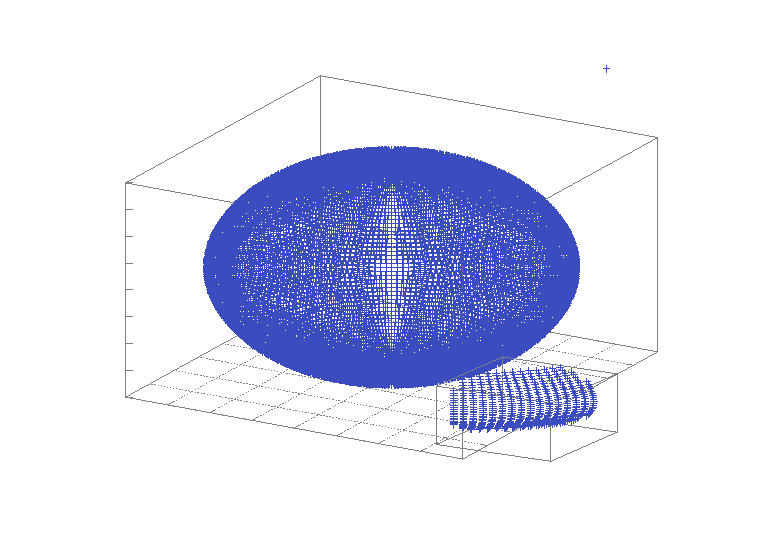
\includegraphics{img/tested_positions_zoom}}%
    \gplfronttext
  \end{picture}%
\endgroup

  \caption{Visualisierung der getesteten Positionen}
  \label{fig:pos}
\end{figure}
Für jeden getesteten Radius haben wir Punkte auf der Kugeloberfläche in 2° Auflösung, also insgesamt 32400 Positionen, getestet.
\begin{figure}[H]
  \centering
  % GNUPLOT: LaTeX picture with Postscript
\begingroup
  \makeatletter
  \providecommand\color[2][]{%
    \GenericError{(gnuplot) \space\space\space\@spaces}{%
      Package color not loaded in conjunction with
      terminal option `colourtext'%
    }{See the gnuplot documentation for explanation.%
    }{Either use 'blacktext' in gnuplot or load the package
      color.sty in LaTeX.}%
    \renewcommand\color[2][]{}%
  }%
  \providecommand\includegraphics[2][]{%
    \GenericError{(gnuplot) \space\space\space\@spaces}{%
      Package graphicx or graphics not loaded%
    }{See the gnuplot documentation for explanation.%
    }{The gnuplot epslatex terminal needs graphicx.sty or graphics.sty.}%
    \renewcommand\includegraphics[2][]{}%
  }%
  \providecommand\rotatebox[2]{#2}%
  \@ifundefined{ifGPcolor}{%
    \newif\ifGPcolor
    \GPcolorfalse
  }{}%
  \@ifundefined{ifGPblacktext}{%
    \newif\ifGPblacktext
    \GPblacktexttrue
  }{}%
  % define a \g@addto@macro without @ in the name:
  \let\gplgaddtomacro\g@addto@macro
  % define empty templates for all commands taking text:
  \gdef\gplbacktext{}%
  \gdef\gplfronttext{}%
  \makeatother
  \ifGPblacktext
    % no textcolor at all
    \def\colorrgb#1{}%
    \def\colorgray#1{}%
  \else
    % gray or color?
    \ifGPcolor
      \def\colorrgb#1{\color[rgb]{#1}}%
      \def\colorgray#1{\color[gray]{#1}}%
      \expandafter\def\csname LTw\endcsname{\color{white}}%
      \expandafter\def\csname LTb\endcsname{\color{black}}%
      \expandafter\def\csname LTa\endcsname{\color{black}}%
      \expandafter\def\csname LT0\endcsname{\color[rgb]{1,0,0}}%
      \expandafter\def\csname LT1\endcsname{\color[rgb]{0,1,0}}%
      \expandafter\def\csname LT2\endcsname{\color[rgb]{0,0,1}}%
      \expandafter\def\csname LT3\endcsname{\color[rgb]{1,0,1}}%
      \expandafter\def\csname LT4\endcsname{\color[rgb]{0,1,1}}%
      \expandafter\def\csname LT5\endcsname{\color[rgb]{1,1,0}}%
      \expandafter\def\csname LT6\endcsname{\color[rgb]{0,0,0}}%
      \expandafter\def\csname LT7\endcsname{\color[rgb]{1,0.3,0}}%
      \expandafter\def\csname LT8\endcsname{\color[rgb]{0.5,0.5,0.5}}%
    \else
      % gray
      \def\colorrgb#1{\color{black}}%
      \def\colorgray#1{\color[gray]{#1}}%
      \expandafter\def\csname LTw\endcsname{\color{white}}%
      \expandafter\def\csname LTb\endcsname{\color{black}}%
      \expandafter\def\csname LTa\endcsname{\color{black}}%
      \expandafter\def\csname LT0\endcsname{\color{black}}%
      \expandafter\def\csname LT1\endcsname{\color{black}}%
      \expandafter\def\csname LT2\endcsname{\color{black}}%
      \expandafter\def\csname LT3\endcsname{\color{black}}%
      \expandafter\def\csname LT4\endcsname{\color{black}}%
      \expandafter\def\csname LT5\endcsname{\color{black}}%
      \expandafter\def\csname LT6\endcsname{\color{black}}%
      \expandafter\def\csname LT7\endcsname{\color{black}}%
      \expandafter\def\csname LT8\endcsname{\color{black}}%
    \fi
  \fi
    \setlength{\unitlength}{0.0500bp}%
    \ifx\gptboxheight\undefined%
      \newlength{\gptboxheight}%
      \newlength{\gptboxwidth}%
      \newsavebox{\gptboxtext}%
    \fi%
    \setlength{\fboxrule}{0.5pt}%
    \setlength{\fboxsep}{1pt}%
\begin{picture}(7200.00,5040.00)%
    \gplgaddtomacro\gplbacktext{%
      \colorrgb{0.50,0.50,0.50}%
      \put(814,704){\makebox(0,0)[r]{\strut{}$0.5$}}%
      \colorrgb{0.50,0.50,0.50}%
      \put(814,1213){\makebox(0,0)[r]{\strut{}$1$}}%
      \colorrgb{0.50,0.50,0.50}%
      \put(814,1722){\makebox(0,0)[r]{\strut{}$1.5$}}%
      \colorrgb{0.50,0.50,0.50}%
      \put(814,2231){\makebox(0,0)[r]{\strut{}$2$}}%
      \colorrgb{0.50,0.50,0.50}%
      \put(814,2740){\makebox(0,0)[r]{\strut{}$2.5$}}%
      \colorrgb{0.50,0.50,0.50}%
      \put(814,3248){\makebox(0,0)[r]{\strut{}$3$}}%
      \colorrgb{0.50,0.50,0.50}%
      \put(814,3757){\makebox(0,0)[r]{\strut{}$3.5$}}%
      \colorrgb{0.50,0.50,0.50}%
      \put(814,4266){\makebox(0,0)[r]{\strut{}$4$}}%
      \colorrgb{0.50,0.50,0.50}%
      \put(814,4775){\makebox(0,0)[r]{\strut{}$4.5$}}%
      \colorrgb{0.50,0.50,0.50}%
      \put(946,484){\makebox(0,0){\strut{}$0.2$}}%
      \colorrgb{0.50,0.50,0.50}%
      \put(1597,484){\makebox(0,0){\strut{}$0.4$}}%
      \colorrgb{0.50,0.50,0.50}%
      \put(2248,484){\makebox(0,0){\strut{}$0.6$}}%
      \colorrgb{0.50,0.50,0.50}%
      \put(2898,484){\makebox(0,0){\strut{}$0.8$}}%
      \colorrgb{0.50,0.50,0.50}%
      \put(3549,484){\makebox(0,0){\strut{}$1$}}%
      \colorrgb{0.50,0.50,0.50}%
      \put(4200,484){\makebox(0,0){\strut{}$1.2$}}%
      \colorrgb{0.50,0.50,0.50}%
      \put(4851,484){\makebox(0,0){\strut{}$1.4$}}%
      \colorrgb{0.50,0.50,0.50}%
      \put(5501,484){\makebox(0,0){\strut{}$1.6$}}%
      \colorrgb{0.50,0.50,0.50}%
      \put(6152,484){\makebox(0,0){\strut{}$1.8$}}%
      \colorrgb{0.50,0.50,0.50}%
      \put(6803,484){\makebox(0,0){\strut{}$2$}}%
    }%
    \gplgaddtomacro\gplfronttext{%
      \csname LTb\endcsname%
      \put(176,2739){\rotatebox{-270}{\makebox(0,0){\strut{}Durchschnittliche Abweichung [°]}}}%
      \put(3874,154){\makebox(0,0){\strut{}Radius der Kugel [m]}}%
      \csname LTb\endcsname%
      \put(5816,4602){\makebox(0,0)[r]{\strut{}Durchschnittliche Abweichung}}%
    }%
    \gplbacktext
    \put(0,0){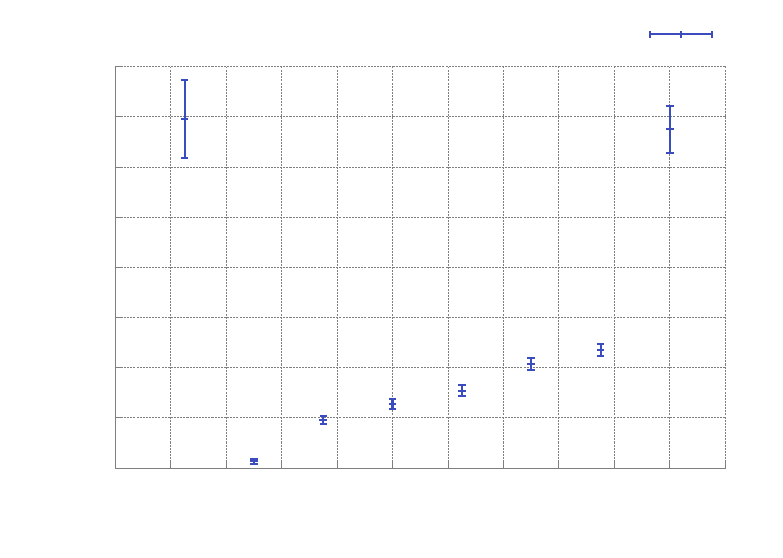
\includegraphics{pos_sweep}}%
    \gplfronttext
  \end{picture}%
\endgroup

  \caption{Genauigkeit für verschiedene Abstände}
  \label{fig:pos_sweep}
\end{figure}
Bei einem Radius von $0.25m$ gibt es einen Ausreißer mit $3.97743^\circ \pm 0.387624^\circ$, da sich die Positionen innerhalb des Tetraeders befinden. Bis $1.75m$ bleibt die Abweichung deutlich unter $2^\circ$, ist also deutlich besser als beim Menschen. Dieser kann auf sehr kurze Distanzen zwischen $10cm$ und $40cm$ gerade einmal mit $3^\circ$ Genauigkeit die Richtung bestimmen. \cite{middlebrooks1991sound}
Um die Abhängigkeit der Genauigkeit der Richtungsbestimmung von der Frequenz zu untersuchen haben wir die Schallquellen wieder auf einer Kugeloberfläche mit $2^\circ$ Auflösung platziert und haben anstelle des Radius die Frequenz variiert. Für den Radius haben wir $1.4m$ gewählt.
\begin{figure}[H]
  \centering
  % GNUPLOT: LaTeX picture with Postscript
\begingroup
  \makeatletter
  \providecommand\color[2][]{%
    \GenericError{(gnuplot) \space\space\space\@spaces}{%
      Package color not loaded in conjunction with
      terminal option `colourtext'%
    }{See the gnuplot documentation for explanation.%
    }{Either use 'blacktext' in gnuplot or load the package
      color.sty in LaTeX.}%
    \renewcommand\color[2][]{}%
  }%
  \providecommand\includegraphics[2][]{%
    \GenericError{(gnuplot) \space\space\space\@spaces}{%
      Package graphicx or graphics not loaded%
    }{See the gnuplot documentation for explanation.%
    }{The gnuplot epslatex terminal needs graphicx.sty or graphics.sty.}%
    \renewcommand\includegraphics[2][]{}%
  }%
  \providecommand\rotatebox[2]{#2}%
  \@ifundefined{ifGPcolor}{%
    \newif\ifGPcolor
    \GPcolorfalse
  }{}%
  \@ifundefined{ifGPblacktext}{%
    \newif\ifGPblacktext
    \GPblacktexttrue
  }{}%
  % define a \g@addto@macro without @ in the name:
  \let\gplgaddtomacro\g@addto@macro
  % define empty templates for all commands taking text:
  \gdef\gplbacktext{}%
  \gdef\gplfronttext{}%
  \makeatother
  \ifGPblacktext
    % no textcolor at all
    \def\colorrgb#1{}%
    \def\colorgray#1{}%
  \else
    % gray or color?
    \ifGPcolor
      \def\colorrgb#1{\color[rgb]{#1}}%
      \def\colorgray#1{\color[gray]{#1}}%
      \expandafter\def\csname LTw\endcsname{\color{white}}%
      \expandafter\def\csname LTb\endcsname{\color{black}}%
      \expandafter\def\csname LTa\endcsname{\color{black}}%
      \expandafter\def\csname LT0\endcsname{\color[rgb]{1,0,0}}%
      \expandafter\def\csname LT1\endcsname{\color[rgb]{0,1,0}}%
      \expandafter\def\csname LT2\endcsname{\color[rgb]{0,0,1}}%
      \expandafter\def\csname LT3\endcsname{\color[rgb]{1,0,1}}%
      \expandafter\def\csname LT4\endcsname{\color[rgb]{0,1,1}}%
      \expandafter\def\csname LT5\endcsname{\color[rgb]{1,1,0}}%
      \expandafter\def\csname LT6\endcsname{\color[rgb]{0,0,0}}%
      \expandafter\def\csname LT7\endcsname{\color[rgb]{1,0.3,0}}%
      \expandafter\def\csname LT8\endcsname{\color[rgb]{0.5,0.5,0.5}}%
    \else
      % gray
      \def\colorrgb#1{\color{black}}%
      \def\colorgray#1{\color[gray]{#1}}%
      \expandafter\def\csname LTw\endcsname{\color{white}}%
      \expandafter\def\csname LTb\endcsname{\color{black}}%
      \expandafter\def\csname LTa\endcsname{\color{black}}%
      \expandafter\def\csname LT0\endcsname{\color{black}}%
      \expandafter\def\csname LT1\endcsname{\color{black}}%
      \expandafter\def\csname LT2\endcsname{\color{black}}%
      \expandafter\def\csname LT3\endcsname{\color{black}}%
      \expandafter\def\csname LT4\endcsname{\color{black}}%
      \expandafter\def\csname LT5\endcsname{\color{black}}%
      \expandafter\def\csname LT6\endcsname{\color{black}}%
      \expandafter\def\csname LT7\endcsname{\color{black}}%
      \expandafter\def\csname LT8\endcsname{\color{black}}%
    \fi
  \fi
    \setlength{\unitlength}{0.0500bp}%
    \ifx\gptboxheight\undefined%
      \newlength{\gptboxheight}%
      \newlength{\gptboxwidth}%
      \newsavebox{\gptboxtext}%
    \fi%
    \setlength{\fboxrule}{0.5pt}%
    \setlength{\fboxsep}{1pt}%
\begin{picture}(7200.00,5040.00)%
    \gplgaddtomacro\gplbacktext{%
      \colorrgb{0.50,0.50,0.50}%
      \put(682,704){\makebox(0,0)[r]{\strut{}$0$}}%
      \colorrgb{0.50,0.50,0.50}%
      \put(682,1254){\makebox(0,0)[r]{\strut{}$5$}}%
      \colorrgb{0.50,0.50,0.50}%
      \put(682,1804){\makebox(0,0)[r]{\strut{}$10$}}%
      \colorrgb{0.50,0.50,0.50}%
      \put(682,2354){\makebox(0,0)[r]{\strut{}$15$}}%
      \colorrgb{0.50,0.50,0.50}%
      \put(682,2905){\makebox(0,0)[r]{\strut{}$20$}}%
      \colorrgb{0.50,0.50,0.50}%
      \put(682,3455){\makebox(0,0)[r]{\strut{}$25$}}%
      \colorrgb{0.50,0.50,0.50}%
      \put(682,4005){\makebox(0,0)[r]{\strut{}$30$}}%
      \colorrgb{0.50,0.50,0.50}%
      \put(682,4555){\makebox(0,0)[r]{\strut{}$35$}}%
      \colorrgb{0.50,0.50,0.50}%
      \put(814,484){\makebox(0,0){\strut{}$0$}}%
      \colorrgb{0.50,0.50,0.50}%
      \put(1563,484){\makebox(0,0){\strut{}$100$}}%
      \colorrgb{0.50,0.50,0.50}%
      \put(2311,484){\makebox(0,0){\strut{}$200$}}%
      \colorrgb{0.50,0.50,0.50}%
      \put(3060,484){\makebox(0,0){\strut{}$300$}}%
      \colorrgb{0.50,0.50,0.50}%
      \put(3809,484){\makebox(0,0){\strut{}$400$}}%
      \colorrgb{0.50,0.50,0.50}%
      \put(4557,484){\makebox(0,0){\strut{}$500$}}%
      \colorrgb{0.50,0.50,0.50}%
      \put(5306,484){\makebox(0,0){\strut{}$600$}}%
      \colorrgb{0.50,0.50,0.50}%
      \put(6054,484){\makebox(0,0){\strut{}$700$}}%
      \colorrgb{0.50,0.50,0.50}%
      \put(6803,484){\makebox(0,0){\strut{}$800$}}%
    }%
    \gplgaddtomacro\gplfronttext{%
      \csname LTb\endcsname%
      \put(176,2629){\rotatebox{-270}{\makebox(0,0){\strut{}Durchschnittliche Abweichung [°]}}}%
      \put(3808,154){\makebox(0,0){\strut{}Frequenz [Hz]}}%
      \csname LTb\endcsname%
      \put(5948,4867){\makebox(0,0)[r]{\strut{}Durchschnittliche Abweichung}}%
    }%
    \gplbacktext
    \put(0,0){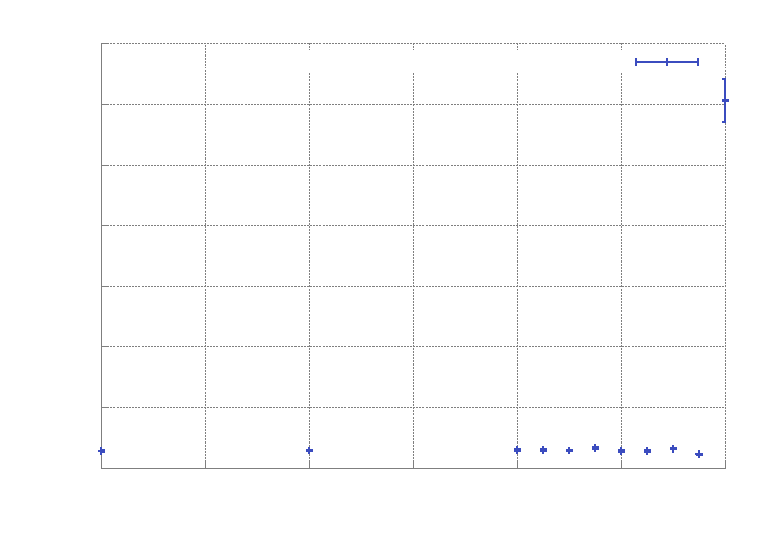
\includegraphics{img/freq_sweep}}%
    \gplfronttext
  \end{picture}%
\endgroup

  \caption{Genauigkeit für verschiedene Frequenzen}
  \label{fig:freq_seep}
\end{figure}
Man sieht, dass die Genauigkeit der Richtungsbestimmung (fast) unabhängig von der Frequenz der Schallquelle ist. Für Frequenzen über $675Hz$ ist die Bedingungen, dass die Abstände der Mikrofone kleiner als die halbe Wellenlänge sein muss, nicht mehr erfüllt.
\subsection{Echtwelt}
In unseren Simulationen hat sich gezeigt, dass unser Verfahren theoretisch sehr genau arbeitet. Um die Genauigkeit in der Echtwelt zu untersuchen haben für acht verschiedene Positionen der Schallquelle die Abweichung der Richtung bestimmt. Diese Messung haben wir in einem mit speziellem Schaumstoff~\cite{BASOTECT} ausgekleideten Raum durchgeführt, um Störungen wie Reflexionen zu minimieren. Der Lautsprecher war jeweils $0.75m$ von dem Zentrum der Mikrofone entfernt.
\begin{minipage}{0.49\linewidth}
\begin{figure}[H]
  \centering
  \resizebox{!}{0.7\textwidth}{% GNUPLOT: LaTeX picture with Postscript
\begingroup
  \makeatletter
  \providecommand\color[2][]{%
    \GenericError{(gnuplot) \space\space\space\@spaces}{%
      Package color not loaded in conjunction with
      terminal option `colourtext'%
    }{See the gnuplot documentation for explanation.%
    }{Either use 'blacktext' in gnuplot or load the package
      color.sty in LaTeX.}%
    \renewcommand\color[2][]{}%
  }%
  \providecommand\includegraphics[2][]{%
    \GenericError{(gnuplot) \space\space\space\@spaces}{%
      Package graphicx or graphics not loaded%
    }{See the gnuplot documentation for explanation.%
    }{The gnuplot epslatex terminal needs graphicx.sty or graphics.sty.}%
    \renewcommand\includegraphics[2][]{}%
  }%
  \providecommand\rotatebox[2]{#2}%
  \@ifundefined{ifGPcolor}{%
    \newif\ifGPcolor
    \GPcolorfalse
  }{}%
  \@ifundefined{ifGPblacktext}{%
    \newif\ifGPblacktext
    \GPblacktexttrue
  }{}%
  % define a \g@addto@macro without @ in the name:
  \let\gplgaddtomacro\g@addto@macro
  % define empty templates for all commands taking text:
  \gdef\gplbacktext{}%
  \gdef\gplfronttext{}%
  \makeatother
  \ifGPblacktext
    % no textcolor at all
    \def\colorrgb#1{}%
    \def\colorgray#1{}%
  \else
    % gray or color?
    \ifGPcolor
      \def\colorrgb#1{\color[rgb]{#1}}%
      \def\colorgray#1{\color[gray]{#1}}%
      \expandafter\def\csname LTw\endcsname{\color{white}}%
      \expandafter\def\csname LTb\endcsname{\color{black}}%
      \expandafter\def\csname LTa\endcsname{\color{black}}%
      \expandafter\def\csname LT0\endcsname{\color[rgb]{1,0,0}}%
      \expandafter\def\csname LT1\endcsname{\color[rgb]{0,1,0}}%
      \expandafter\def\csname LT2\endcsname{\color[rgb]{0,0,1}}%
      \expandafter\def\csname LT3\endcsname{\color[rgb]{1,0,1}}%
      \expandafter\def\csname LT4\endcsname{\color[rgb]{0,1,1}}%
      \expandafter\def\csname LT5\endcsname{\color[rgb]{1,1,0}}%
      \expandafter\def\csname LT6\endcsname{\color[rgb]{0,0,0}}%
      \expandafter\def\csname LT7\endcsname{\color[rgb]{1,0.3,0}}%
      \expandafter\def\csname LT8\endcsname{\color[rgb]{0.5,0.5,0.5}}%
    \else
      % gray
      \def\colorrgb#1{\color{black}}%
      \def\colorgray#1{\color[gray]{#1}}%
      \expandafter\def\csname LTw\endcsname{\color{white}}%
      \expandafter\def\csname LTb\endcsname{\color{black}}%
      \expandafter\def\csname LTa\endcsname{\color{black}}%
      \expandafter\def\csname LT0\endcsname{\color{black}}%
      \expandafter\def\csname LT1\endcsname{\color{black}}%
      \expandafter\def\csname LT2\endcsname{\color{black}}%
      \expandafter\def\csname LT3\endcsname{\color{black}}%
      \expandafter\def\csname LT4\endcsname{\color{black}}%
      \expandafter\def\csname LT5\endcsname{\color{black}}%
      \expandafter\def\csname LT6\endcsname{\color{black}}%
      \expandafter\def\csname LT7\endcsname{\color{black}}%
      \expandafter\def\csname LT8\endcsname{\color{black}}%
    \fi
  \fi
    \setlength{\unitlength}{0.0500bp}%
    \ifx\gptboxheight\undefined%
      \newlength{\gptboxheight}%
      \newlength{\gptboxwidth}%
      \newsavebox{\gptboxtext}%
    \fi%
    \setlength{\fboxrule}{0.5pt}%
    \setlength{\fboxsep}{1pt}%
\begin{picture}(7200.00,5040.00)%
    \gplgaddtomacro\gplbacktext{%
      \colorrgb{0.50,0.50,0.50}%
      \put(946,1067){\makebox(0,0)[r]{\strut{}$-0.6$}}%
      \colorrgb{0.50,0.50,0.50}%
      \put(946,1551){\makebox(0,0)[r]{\strut{}$-0.4$}}%
      \colorrgb{0.50,0.50,0.50}%
      \put(946,2035){\makebox(0,0)[r]{\strut{}$-0.2$}}%
      \colorrgb{0.50,0.50,0.50}%
      \put(946,2520){\makebox(0,0)[r]{\strut{}$0$}}%
      \colorrgb{0.50,0.50,0.50}%
      \put(946,3004){\makebox(0,0)[r]{\strut{}$0.2$}}%
      \colorrgb{0.50,0.50,0.50}%
      \put(946,3488){\makebox(0,0)[r]{\strut{}$0.4$}}%
      \colorrgb{0.50,0.50,0.50}%
      \put(946,3972){\makebox(0,0)[r]{\strut{}$0.6$}}%
      \colorrgb{0.50,0.50,0.50}%
      \put(1166,484){\makebox(0,0){\strut{}$-0.8$}}%
      \colorrgb{0.50,0.50,0.50}%
      \put(1871,484){\makebox(0,0){\strut{}$-0.6$}}%
      \colorrgb{0.50,0.50,0.50}%
      \put(2575,484){\makebox(0,0){\strut{}$-0.4$}}%
      \colorrgb{0.50,0.50,0.50}%
      \put(3280,484){\makebox(0,0){\strut{}$-0.2$}}%
      \colorrgb{0.50,0.50,0.50}%
      \put(3985,484){\makebox(0,0){\strut{}$0$}}%
      \colorrgb{0.50,0.50,0.50}%
      \put(4689,484){\makebox(0,0){\strut{}$0.2$}}%
      \colorrgb{0.50,0.50,0.50}%
      \put(5394,484){\makebox(0,0){\strut{}$0.4$}}%
      \colorrgb{0.50,0.50,0.50}%
      \put(6098,484){\makebox(0,0){\strut{}$0.6$}}%
      \colorrgb{0.50,0.50,0.50}%
      \put(6803,484){\makebox(0,0){\strut{}$0.8$}}%
    }%
    \gplgaddtomacro\gplfronttext{%
      \csname LTb\endcsname%
      \put(176,2519){\rotatebox{-270}{\makebox(0,0){\strut{}y [m]}}}%
      \put(3940,154){\makebox(0,0){\strut{}x [m]}}%
      \csname LTb\endcsname%
      \put(5948,4867){\makebox(0,0)[r]{\strut{}Bestimmte Richtung}}%
      \csname LTb\endcsname%
      \put(5948,4647){\makebox(0,0)[r]{\strut{}Tatsächliche Richtung}}%
    }%
    \gplbacktext
    \put(0,0){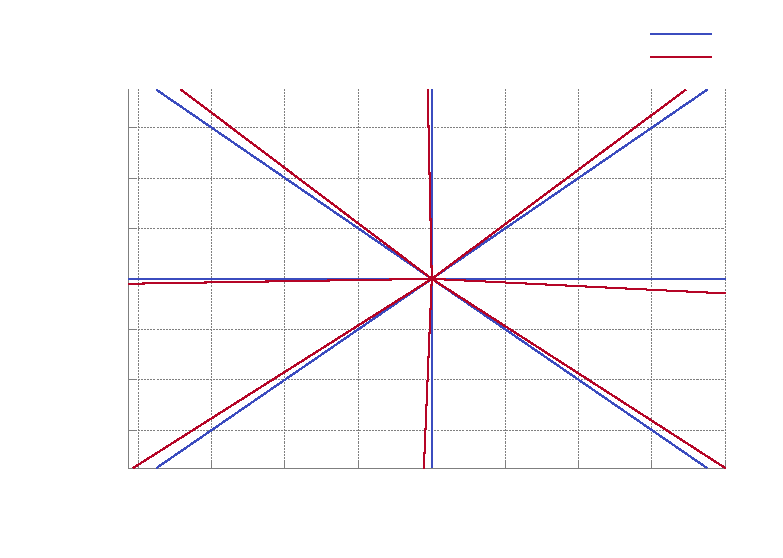
\includegraphics{img/real}}%
    \gplfronttext
  \end{picture}%
\endgroup
}
  \caption{Genauigkeit in der Echtwelt}
  \label{fig:real}
\end{figure}
\end{minipage}\hfill\todo{Diese Bild ist nur ein Platzhalter -> muss noch aufgenommen werden!!!!}%%
\begin{minipage}{0.49\linewidth}
\begin{figure}[H]
  \centering
  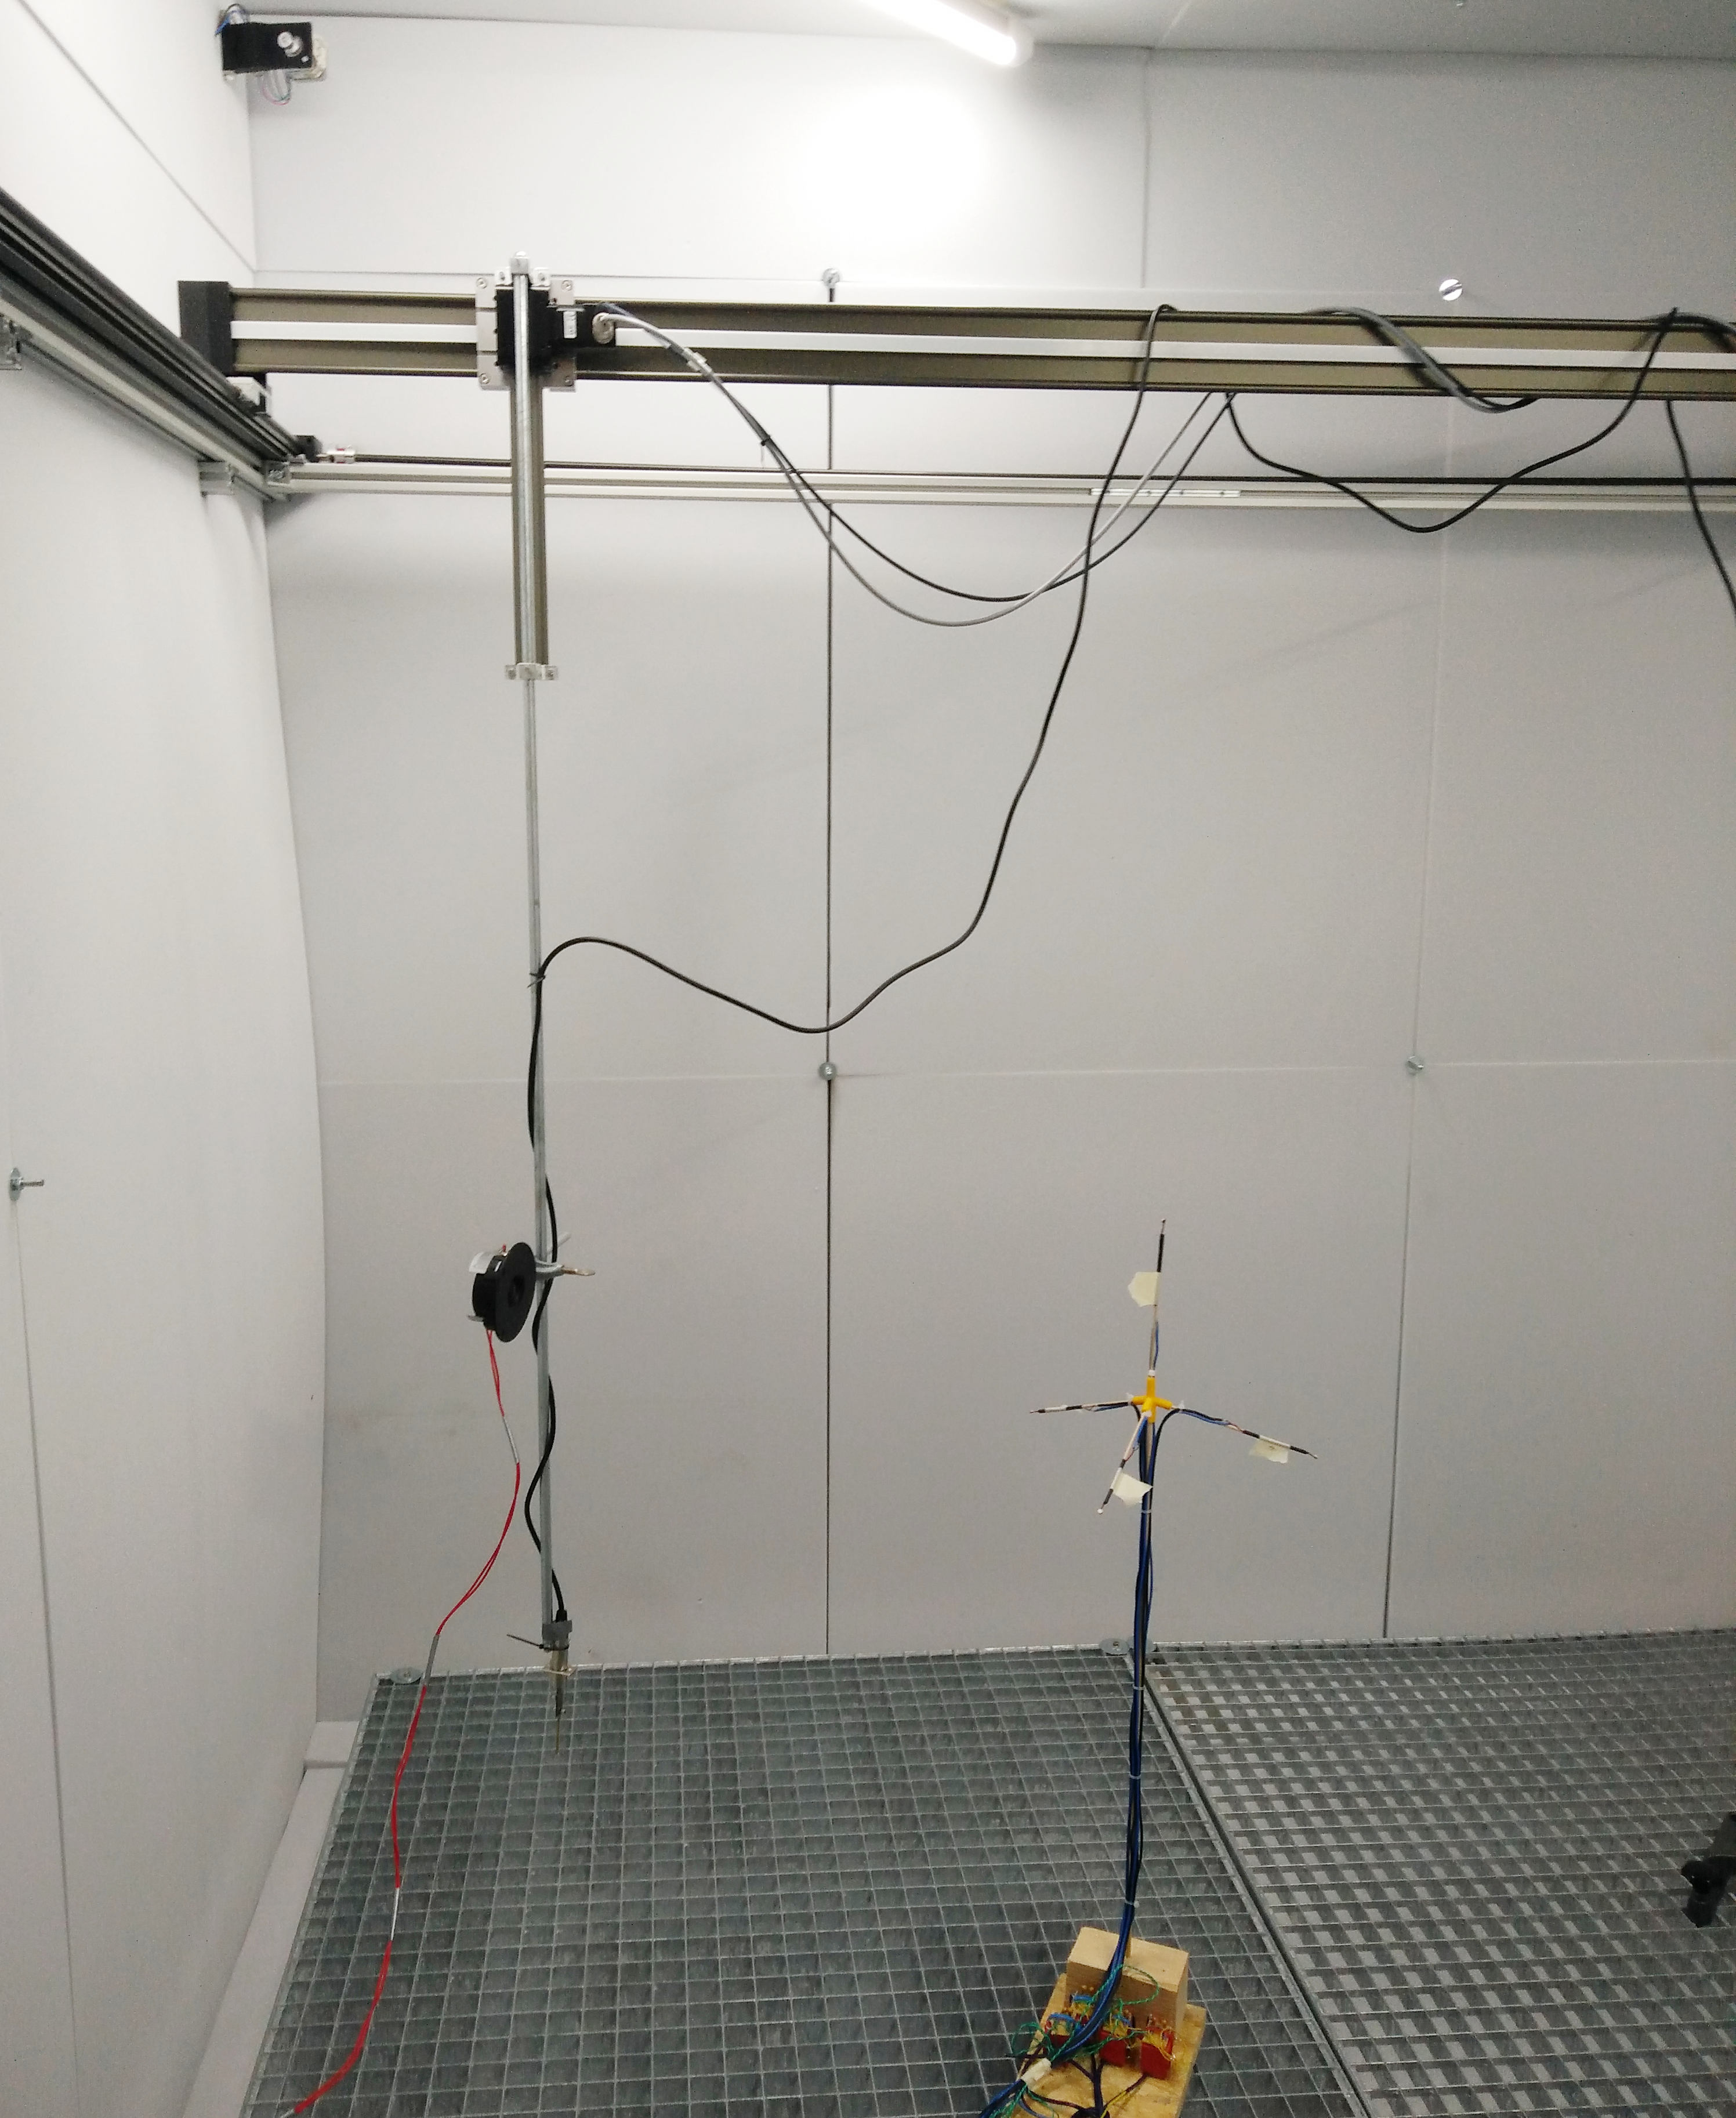
\includegraphics[width=\textwidth]{img/pos_1}
  \caption{Versuchsaufbau zur Messung der Genauigkeit der Richtungsbestimmung in der Schallkammer}
  \label{fig:real_reral}
\end{figure}
\end{minipage}%%
Für die acht verschiedenen Richtungen hatte die Richtungsbestimmung eine Genauigkeit von $3.9^\circ \pm 0.13^\circ$. Allerdings hatte der Lautsprecher bei dem von uns gewählten Abstand eine Größe von $3.2^\circ$, genauer also diese kann die Richtungsbestimmung also nicht sein. Die Richtungsbestimmung mit unserem Verfahren ist also auch in der Echtwelt genauer als der Mensch.
Um die Verwendbarkeit unseres Verfahren auch außerhalb einer Schallkammer zu testen haben wir die Richtungsbestimmung zweier sich unterhaltender Personen untersucht.
\begin{minipage}{0.49\linewidth}
  \begin{figure}[H]
    \centering
    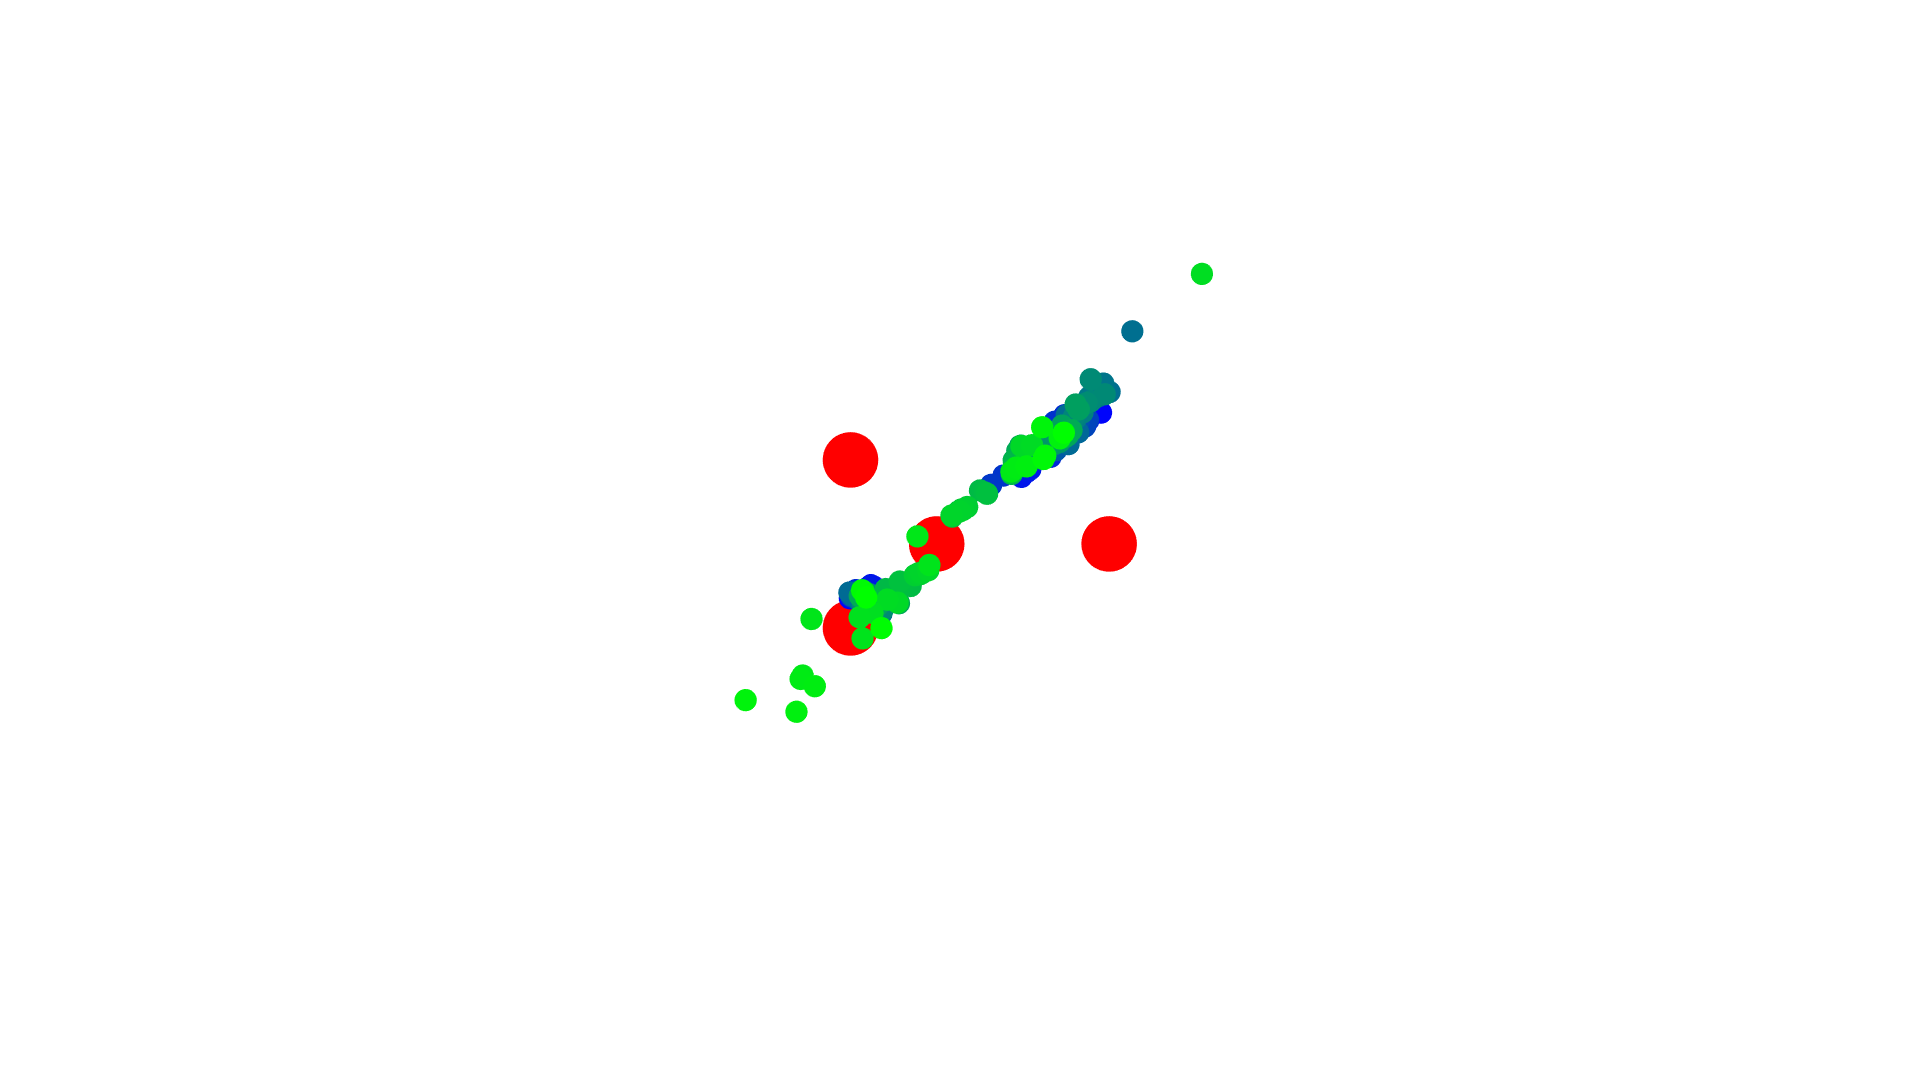
\includegraphics[width=\textwidth]{img/real_real_data}
    \caption{Bestimmte Richtungen}
    \label{fig:real_real_data}
  \end{figure}
\end{minipage}\hfill
\begin{minipage}{0.49\linewidth}
  \begin{figure}[H]
    \centering
    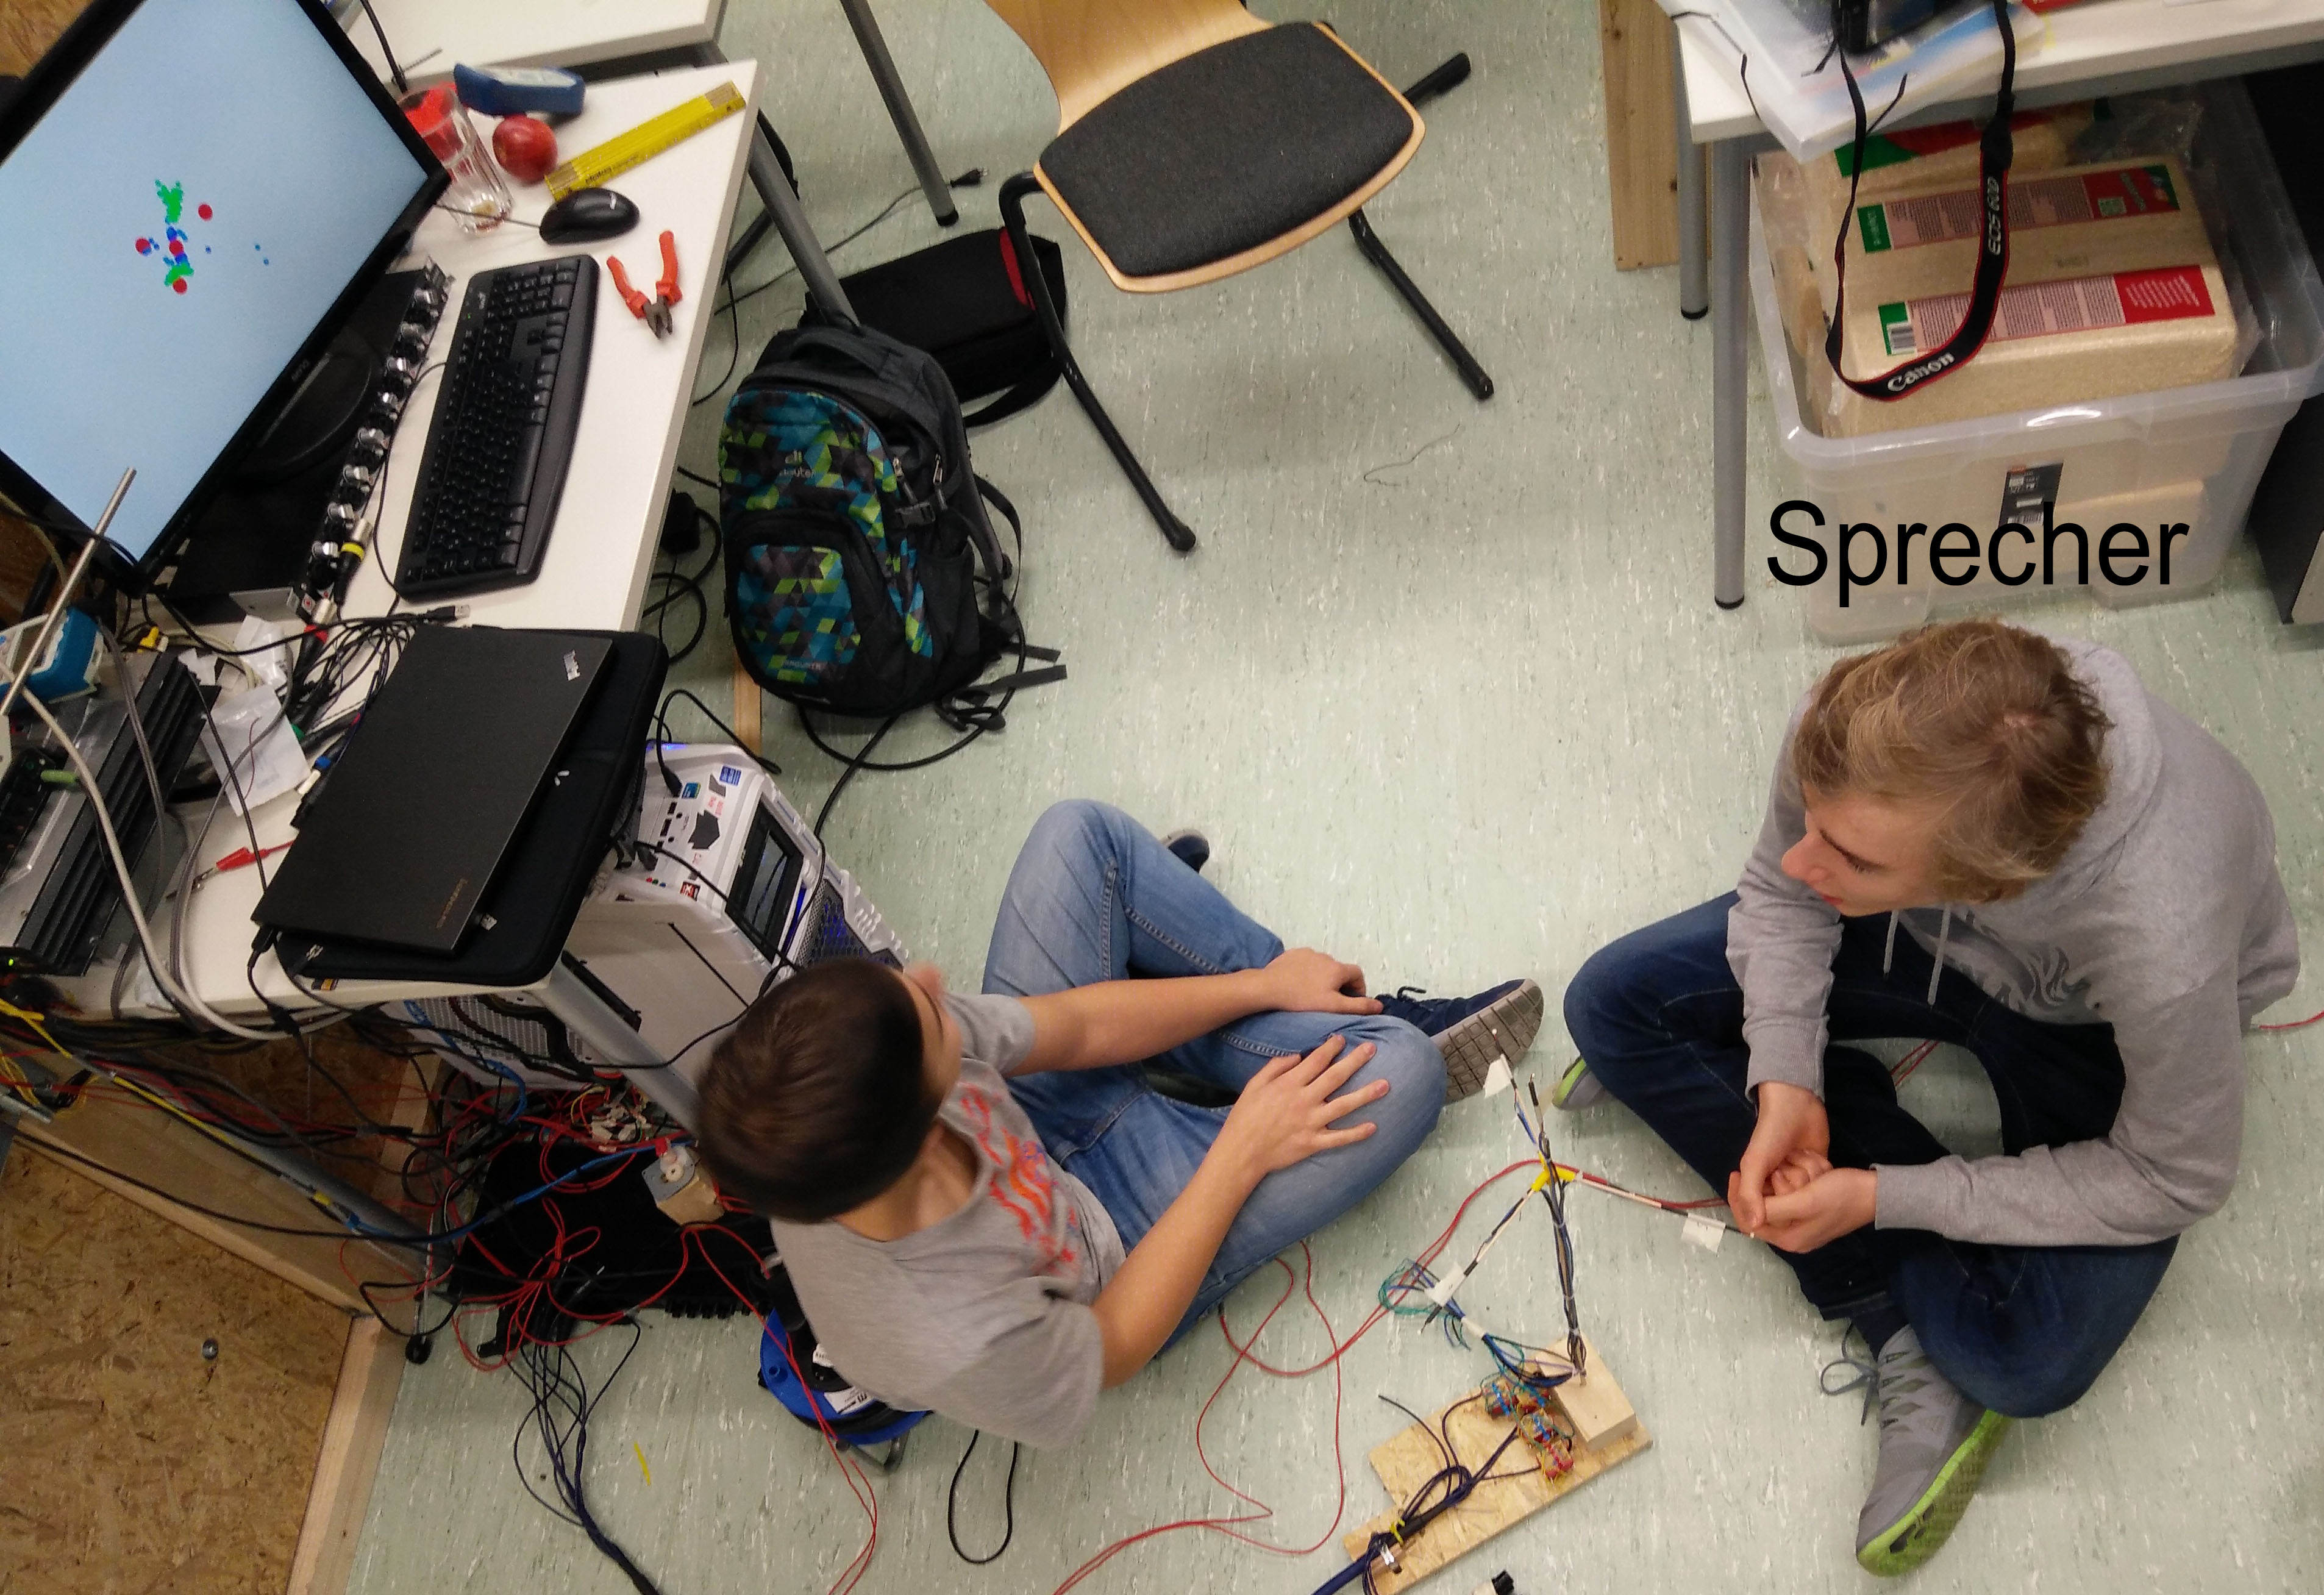
\includegraphics[width=\textwidth]{img/real_real}
    \caption{Tatsächliche Position}
    \label{fig:real_real}
  \end{figure}
\end{minipage}

Man kann erkennen, das die mit unserem Verfahren bestimmte Richtung sehr gut mit der tatsächlichen Richtung übereinstimmt und es auch nur eine sehr geringe Streuung der Richtung gibt. Dies zeigt, das es auch für Echtwelt Situationen bei denen Störungen wie Reflexionen auftreten gut geeignet ist.
    \section{Ausblick}
Unser Verfahren ermöglicht die Richtungsbestimmung mit gerade einmal 4 Mikrofonen. Da unser Verfahren über die Least Squares Methode sehr leicht auf eine beliebige Anzahl von Mikrofonen erweiterbar ist, wollen wir die Genauigkeit und insbesondere die Reichweite der Richtungsbestimmung noch weiter erhöhen, indem wir anstelle von vier Mikrofonen acht Mikrofone verwenden. Dies würde es uns außerdem erlauben, die Richtungsbestimmung unabhängig von der Schallgeschwindigkeit  durchzuführen, indem diese als eine weitere Variable eingeführt wird. Damit würde sich die Genauigkeit der Richtungsbestimmung weiter verbessern.
Weiterhin könnte die Richtungsbestimmung verbessert werden, indem auch die Amplituden mit einbezogen werden. Diese stehen durch die Fourier-Transformation bereits zur Verfügung und könnten ebenfalls zu einer weiteren Verbesserung der Reichweite und Genauigkeit der Richtungsbestimmung beitragen.
Dadurch, dass wir anstatt einer Richtung eigentlich eine Position bestimmen, könnte man unser Verfahren nach weiterer Optimierung auch für die Positionsbestimmung von Schallquellen verwenden.

    \section{Fazit}
Insgesamt ist es uns im Rahmen dieser Jugend-Forscht Arbeit gelungen, ein neues Verfahren zur Richtungsbestimmung von Schallquellen zu entwickeln und zu evaluieren, das gerade einmal vier Mikrofone benötigt, um deutlich besser als der Mensch die Richtung zu bestimmen. Die Implementation unseres Verfahrens ist modular aufgebaut und ermöglicht dadurch eine leichte Integration in bestehende Programme und weitere Verarbeitungs- und Auswertungsschritte. Hierdurch ist es Möglich, das von uns entwickelte System in Technische Anwendungen zu integrieren und somit die Fähigkeit des Richtungshörens zu nutzen.

  \endgroup

  \pagebreak % Quellen und co
  \pagenumbering{roman}
  \setcounter{page}{1}
  \printbibliography
\end{document}